Resulta imposible abarcar el seguimiento de todo el código desarrollado. En esta sección por tanto vamos a exponer la ejecución del proyecto haciendo foco en los casos de uso más representativos de toda la metodología que este trabajo ha desarrollado en su fase de diseño. El resto se expondrá de una forma más gráfica con diagramas que hagan comprensible la estructura y no tanto los detalles de implementación.

Una de las primeras características que cabe resaltar de golang es que no tiene clases ni herencia. como estructura
principal de datos tiene los structs. Si queremos garantizar la encapsulación, sobre todo en los elementos de dominio y aplicación. Garantizar que dichose elementos se creen bajo una misma logica que no se pueda evitar, por ejemplo, declaración inicial de variables de dichos structs que representen las Entities, los Value Objects, etc.

De tal forma que debemos entender que olang sólo expone elementos, ya sea structs, funciones o demás tipos fuera de un módulo si están escritos en Mayuscula. Un módulo son todos los archivos dentro de un mismo directorio.

Por lo tanto una forma de crear una estructura equivalente a una clase es definir una interfaz pública y crear un struct privado que la implemente. los struct pueden implementar metodos pasandose a si mismos por referencia en una funcion. De tal forma se puede ver en\ref{fig:golang class equivalent}

\begin{figure}[H]
    \centering
    \begin{lstlisting}[label={lst:lstlisting}]
        type ClassName interface {
            GetVariable() string
            GetAnotherVariable() string
            SetVariable(newValue string)
        }

        type className struct {
            variable string
            anotherVariable string
        }

        func NewClassName(variable string) (ClassName, error) {
            if variable == "invalid" {
                return nil, errors.New("error")
            }
            return &className{variable,"DEFAULT"},nil
        }

        func (c *className) GetVariable() string {
            return c.variable
        }

        func (c *className) GetAnotherVariable() string {
            return c.anotherVariable
        }

        func (c *className) SetVariable(newValue string) {
            c.variable = newValue
        }
    \end{lstlisting}
    \caption{fig:golang class equivalent}\label{fig:golang class equivalent}
\end{figure}

Donde podemos ver que \textbf{C}lassName interface la 'C' es mayúscula exponiendolo al exterior del módulo y \textbf{c}lassName struct en minuscula encapsulándolo.
lo cual resulta en un diagrama UML\ref{fig: uml Diagram Class Equivalent in Golang}

\begin{figure}[H]
    \centering
    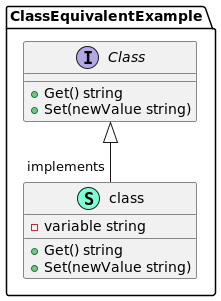
\includegraphics[height=0.3\textheight]{./part/Proyecto_ejecutivo/memoria_constructiva/ClassEquivalentInGolang}
    \caption{UML diagram: Class equivalent in Golang}\label{fig: uml Diagram Class Equivalent in Golang}
\end{figure}

por qué es importante concebir esta estructura:

\begin{itemize}
    \item Evitamos la instanciación no consistente, lo cual solo se garantiza a traves del método si exportado NewClass
    \item evitamos accesos no deseados al seteo de variables. Si las pusieramos publicas seria posible. esto es de vital importancia a la hora de establecer el concepto de inmutabilidad en la que se basan los value objects.
    \item otro punto de limpieza que aporta, es a la hora de gestionar errores en golang. Si en cualquier punto queremos devolver como resultado de una función un objeto o el error, característica de golang que permite devolver varios elementos como resultado, Nos veríamos obligados a instanciar el objeto con contenido vacío y el error, creando un elemento inconsistente sólo por exigencias del lenguaje. De esta forma, podemos poner como parámetro de retorno dicha interfaz que sí puede ser null.
\end{itemize}

como contrapartida tenemos que escribir más codigo. poniendo como comparación una clase java o C++ no podemos decir que en cantidad de lineas escritas se aumente o disminuya. En cuestión de conceptos aprendidos en Golang sólamente trabaja con interfaces y structs contra el concepto de clase y herencia.

Una vez presentado este concepto clave de golang pasamos a exponer el código que se ha ejecutado. Siendo programas extensos hemos decidido escoger el caso de uso más extenso el cuál incluye la gestión de los eventos y el proceso de intercomunicación. También expondremos expondremos el programa de control.

Vamos a dividir esta sección en:
\begin{itemize}
    \item CreateTaskUseCase
    \item TaskEventHandler
\end{itemize}

Que son los puntos que han presentado mayor complejidad.

\subsubsection{CreateTaskUseCase}
    
El codigo de colores utilizado en los diagramas de esta seccion se refieren al equivalente a clase en golang en azul y a las interfaces puras en turquesa  y a los structs en marron

%El tipico diagráma cuando se habla de arquitectura hexagonal es tal y como se muestra en la figura\ref{fig:hexagonalDiagram} Si bien consideramos que no tiene mucho sentido y de cara a la parte didáctica confunde, ya que el hexágono es una simple licencia estética. en el caso de existir más puertos de salida y entrada que los representados el hexágono pierde todo el sentido y cuando se enfrenta por primera vez este diagrama se tiende a intentar descifrar el sentído del hexagono.
%
%\begin{figure}[H]
%    \centering
%    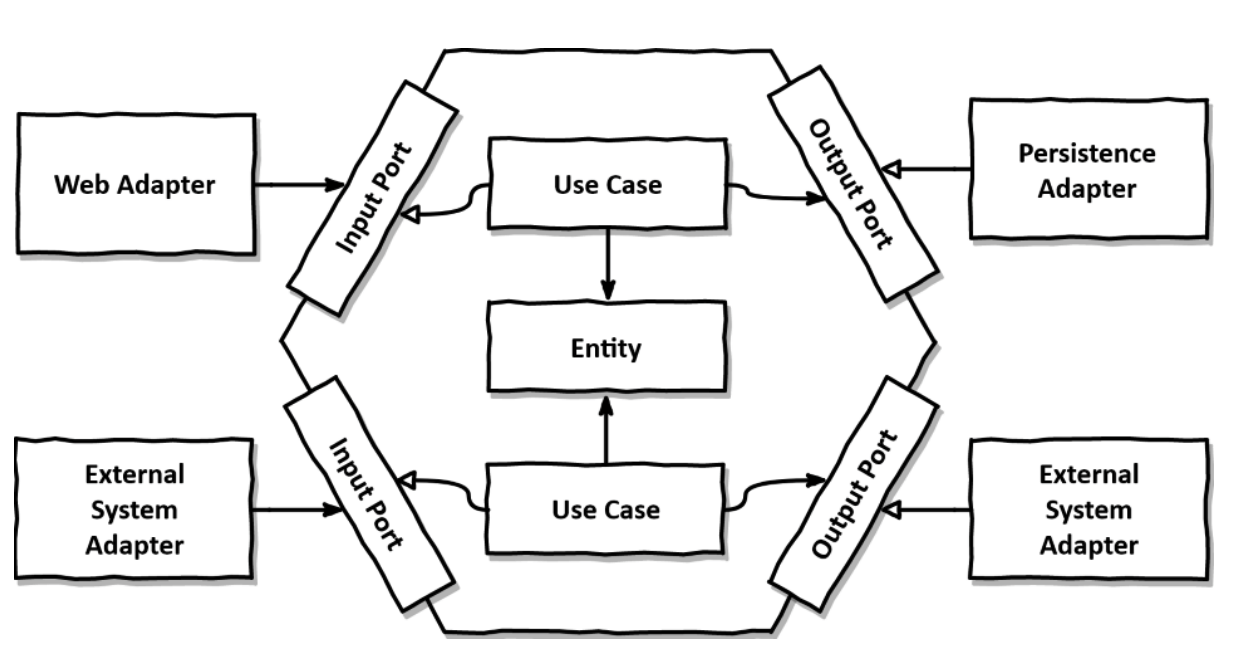
\includegraphics[height=0.3\textheight]{./part/Ejecucion/Seguimiento/CreateTaskUseCase/img/HexagonalDiagram}
%    \caption{Hexagonal architecture diagram\cite{TomHombergs2019GYHD}}\label{fig:hexagonalDiagram}
%\end{figure}

Tomando como referencia \ref{fig:hexagonalDiagram} el diagrmaa tipico de una arquitectura hexagonal, en nuestro caso si intercambiamos ExternalSystemAdapter por nuestro Dispatcher de eventos e introducimos servicios de dominio entre el caso de uso y la Entidad tendremos nuestro esquema de alto nivel de nuestra arquitectura hexagonal. El esbozo de este diagrama lo podemos encontrar en la figura\ref{fig:CreateTaskHexagonalDiagram} Como vemos no tiene tanto sentido el dibujo ya que hay puertos de salida que se convierten en puertos de entrada como es el dispatcher y cuando queremos quitar lógica de negocio del caso de uso mediante servicios de dominio que impidan el acceso directo a los repositorios de persistencia dicho diagrama se va quedando pequeño. Es perferible diagramas UML tal y comose muestra en\ref{fig:createTaskUseCaseArchitecture}


\begin{figure}[H]
    \centering
    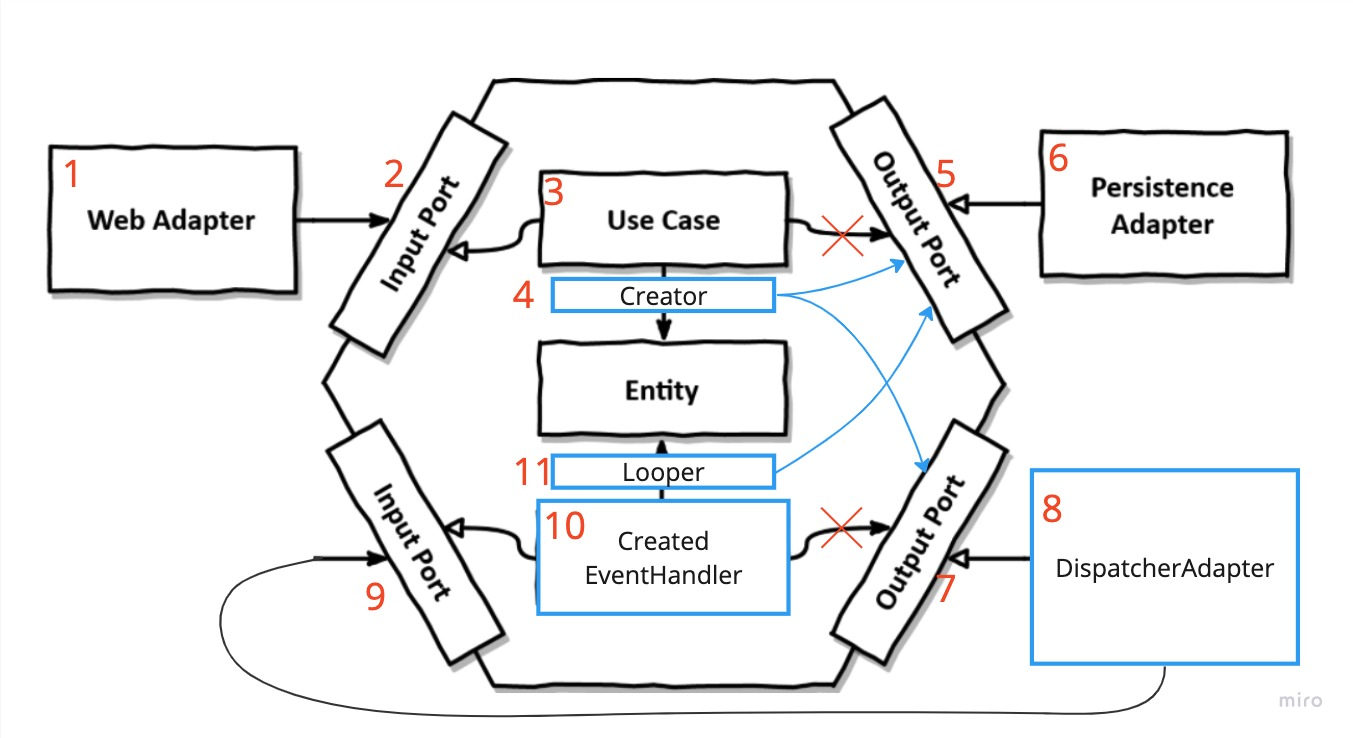
\includegraphics[height=0.3\textheight]{./part/Ejecucion/Seguimiento/CreateTaskUseCase/img/CreateTaskHexagonalDiagram}
    \caption{Hexagonal architecture diagram}\label{fig:CreateTaskHexagonalDiagram}
\end{figure}

\begin{figure}[H]
    \centering
    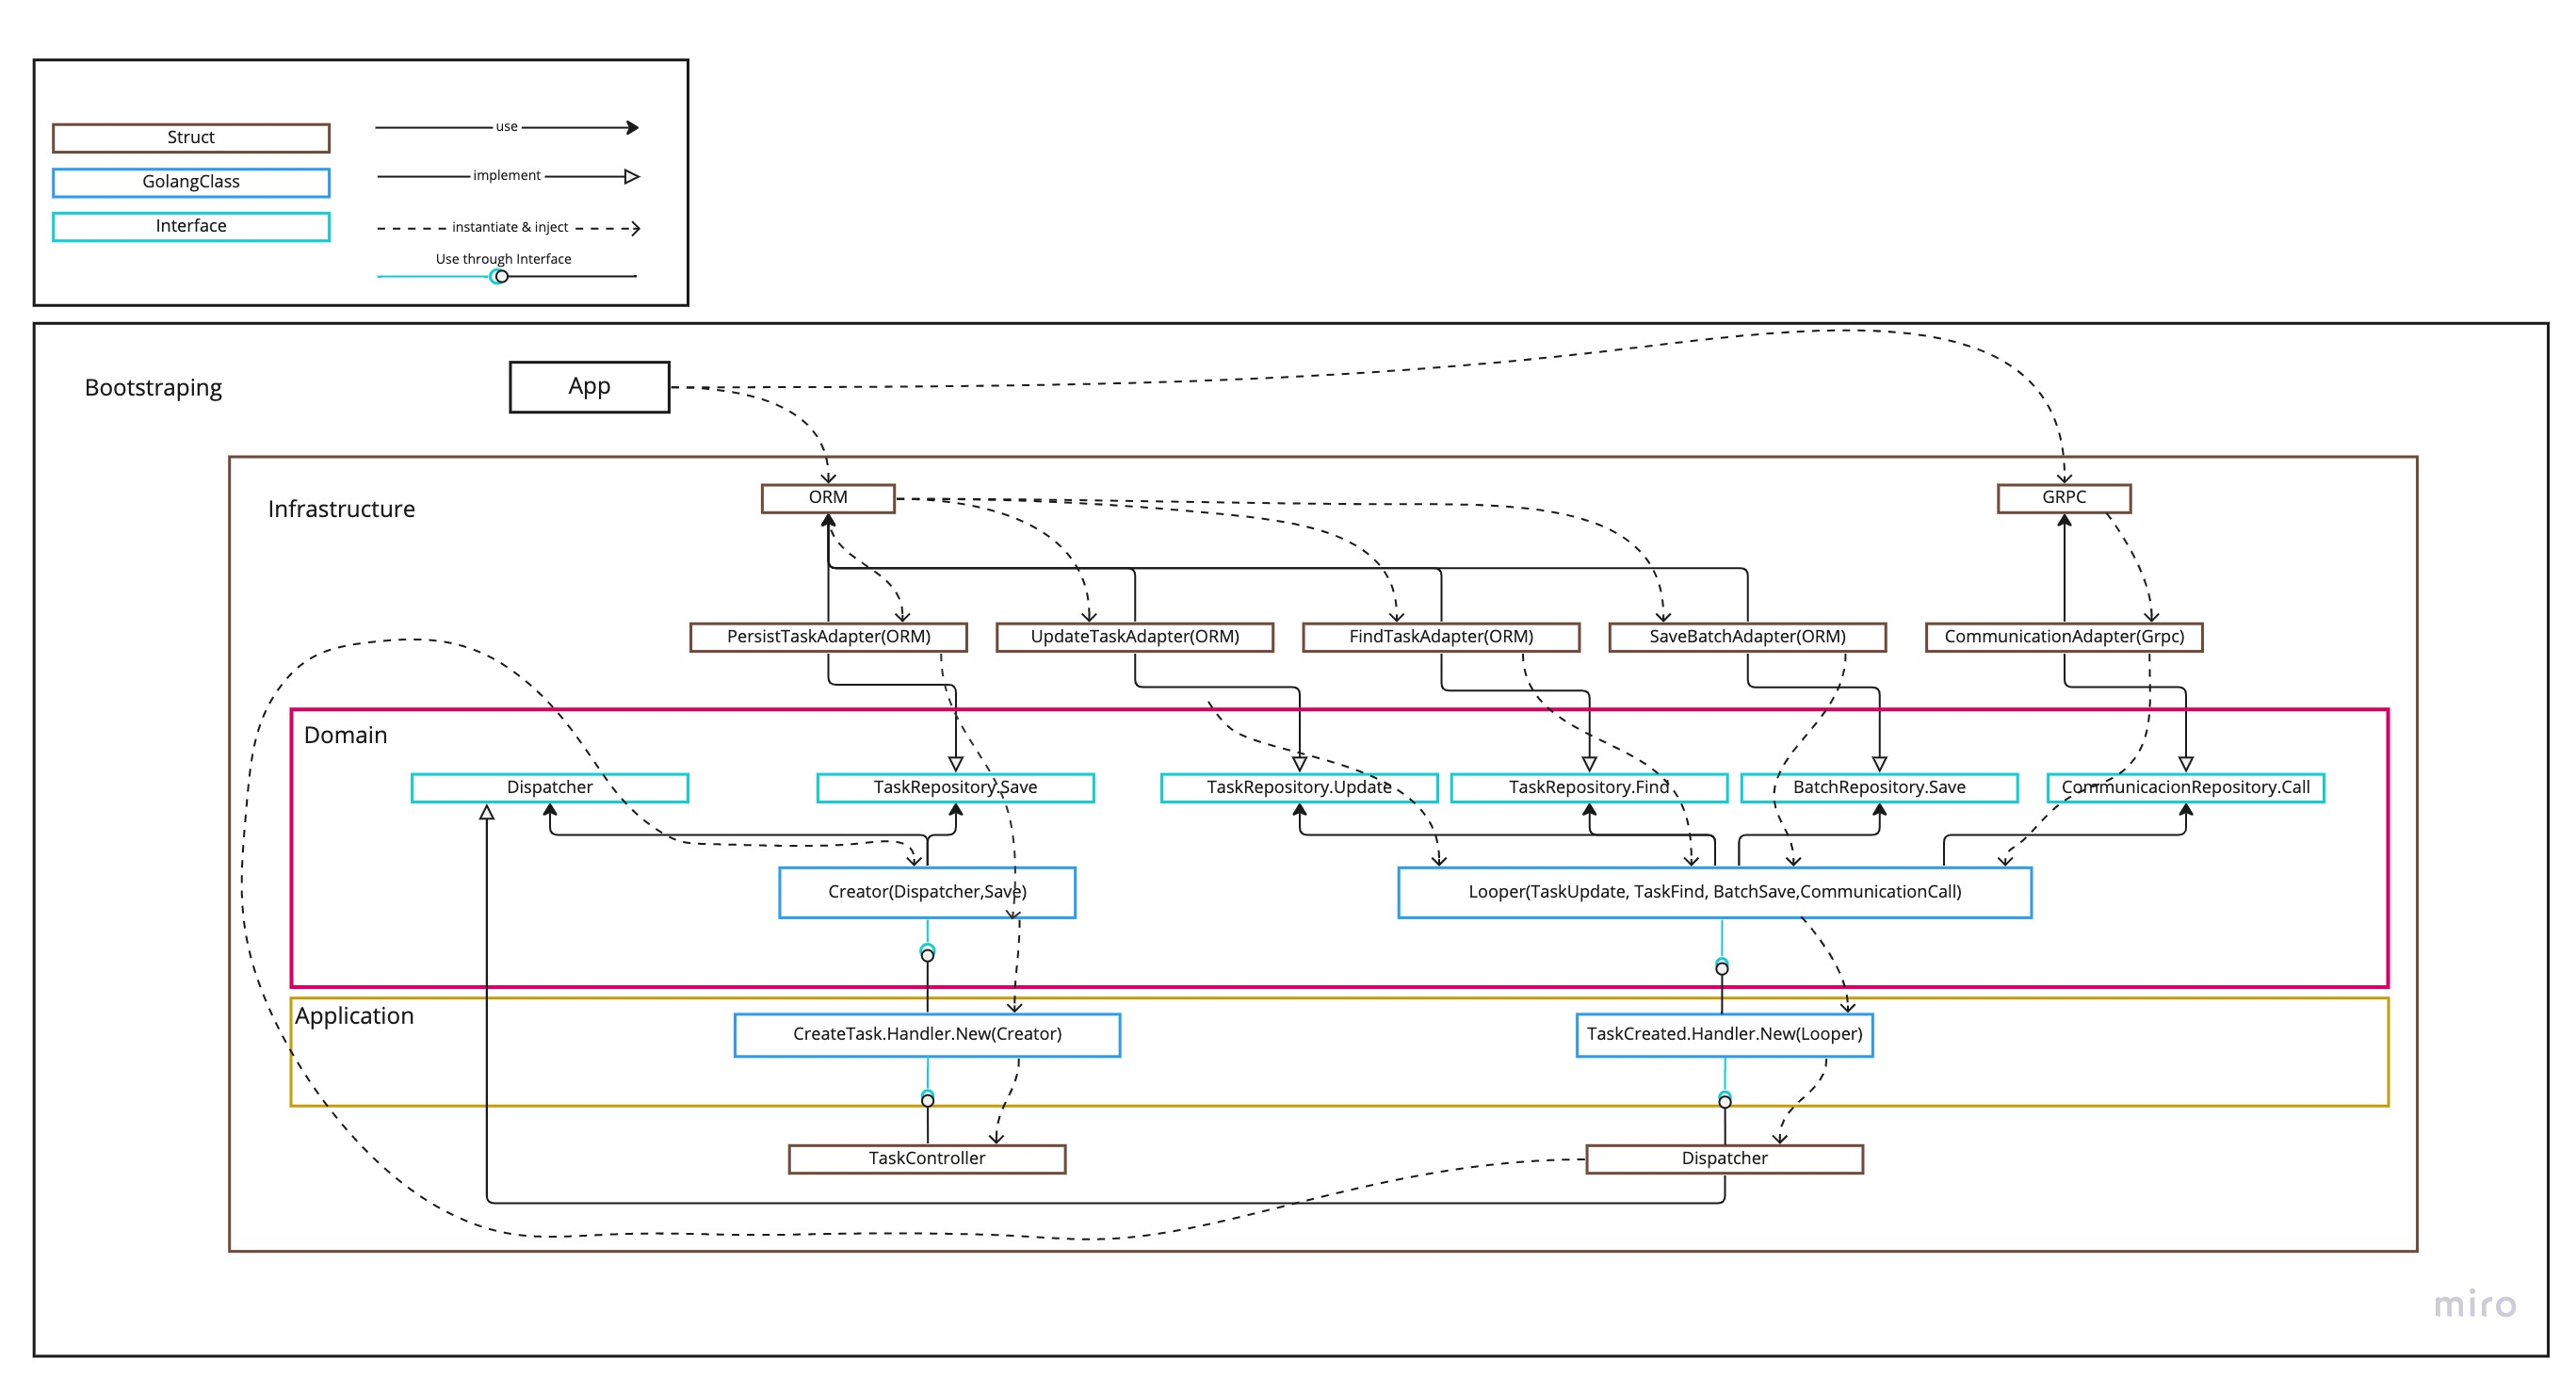
\includegraphics[height=0.3\textheight]{./part/Ejecucion/Seguimiento/CreateTaskUseCase/img/createTaskUseCaseArchitecture}
    \caption{CreateTaskUseCase hexagonal architecture diagram}\label{fig:createTaskUseCaseArchitecture}
\end{figure}

Acercandonos más al código podemos ver en el diagrama \ref{fig:createTaskUseCaseArchitectureFolderStructure} cómo es el uso entre los componentes que exísten en la estructrura de carpetas.

\begin{figure}[H]
    \centering
    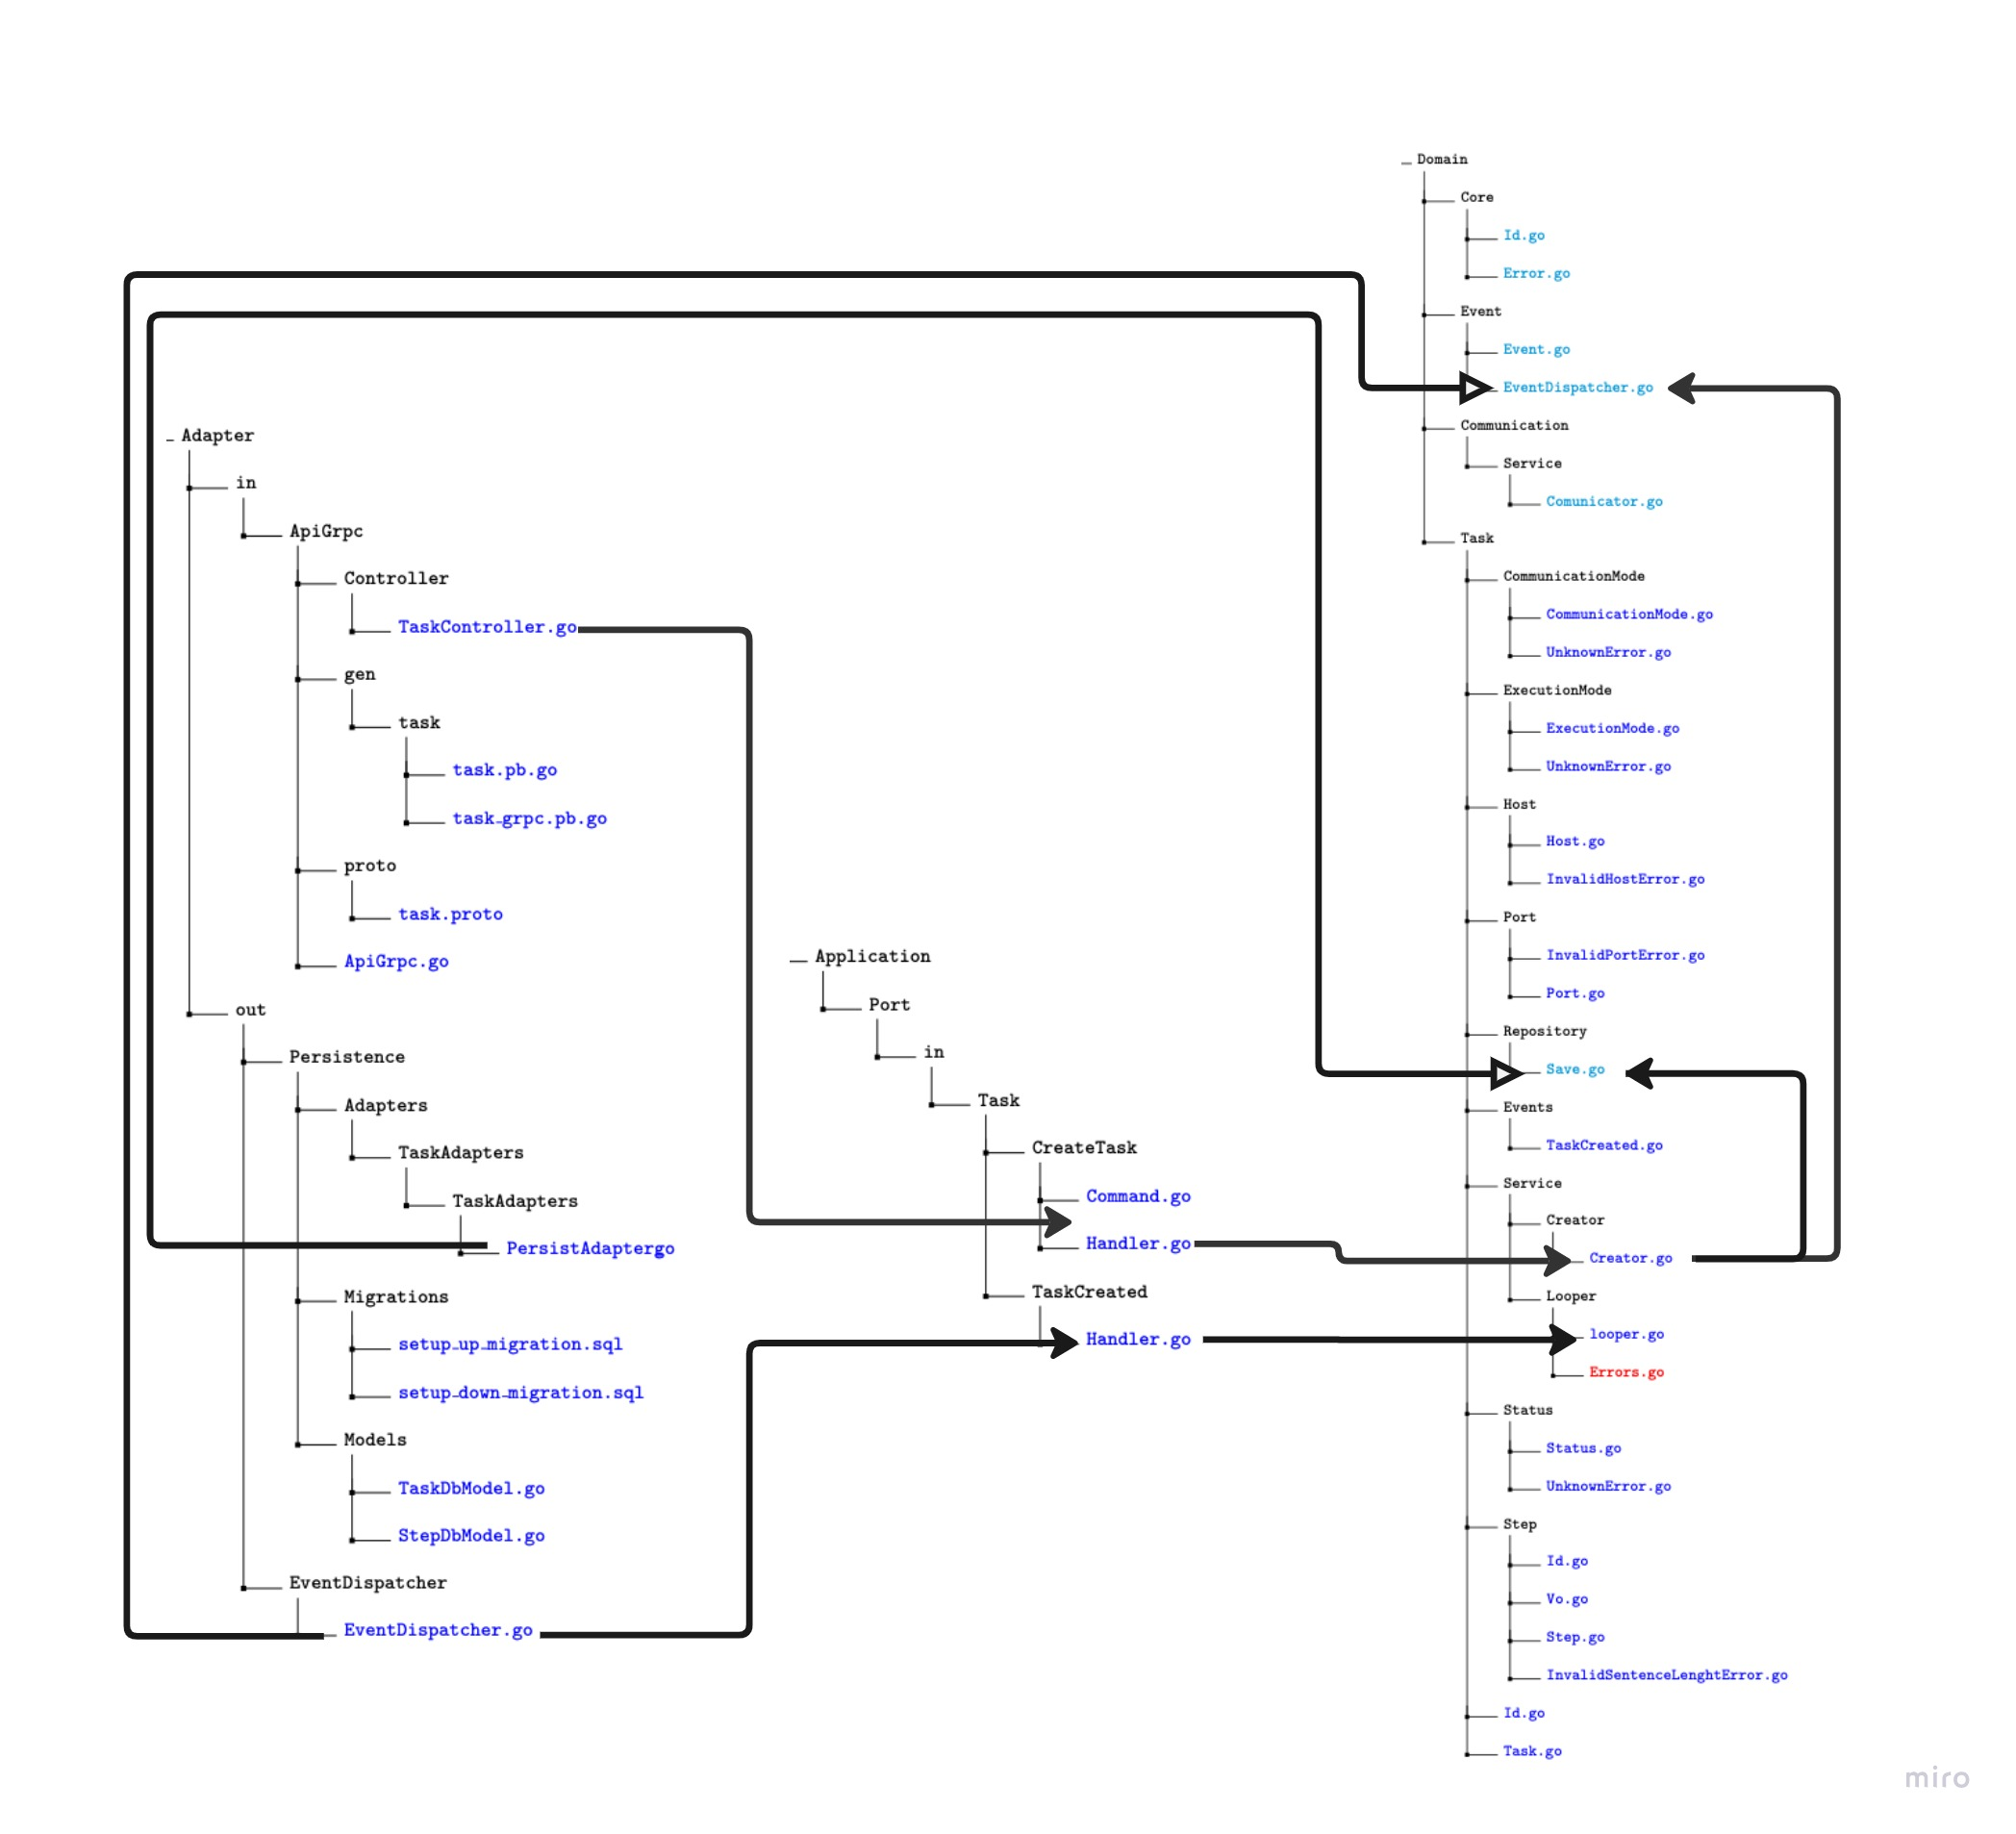
\includegraphics[height=0.5\textheight]{./part/Ejecucion/Seguimiento/CreateTaskUseCase/img/PFM - CreateUseCaseFolderStructure}
    \caption{CreateTaskUseCase folder Structure}\label{fig:createTaskUseCaseArchitectureFolderStructure}
\end{figure}

%Un punto interesante a comentar es el concepto de la estrategia de mapping que hay entre capas. Cada capa requiere sus objetos de trabajo. Tal y como sale descrito en \cite{TomHombergs2019GYHD} Tenemos tantas estratégias como atajos dentro de este paradigma queramos asumir. podemos ver en la figura \ref{fig:mapping types} Los tipos de mapping que se documentan en este libro:
%\begin{itemize}
%    \item The NoMapping Strategy
%    \item The Two-Way MappingStrategy
%    \item The Full MappingStrategy
%    \item The One-Way MappingStrategy
%\end{itemize}

Con respecto a la estrategia de mapping Golang nos permite hacer un full strategy casi por defecto porque al necesitar la implementaci'on de clase para garantizar la cohesión ya estamos utilizando interfaces para todas las clases. Así que en este caso utilizamos un fullMapping adaptado. lo cierto es que las versiones intermedias son todas las combinaciones posibles.

De cara a decidir extraemos la recomendacion de  \cite{TomHombergs2019GYHD}:"
we might start with a simple strategy that allows us to quickly evolve the code and later move to a more complex one that helps us to better decouple the layers.
In order to decide which strategy to use when, we need to agree upon a set of guidelines within the team. These guidelines should answer the question which mapping strategy should be the first choice in which situation. They should also answer why they are first choice so that we’re able to evaluate if those reasons still apply after some time."

Al final se trata de tomar una decisión en equipo, documentar las razones y ser consistentes. Reevaluar las razones ante un reto que las ponga a prueba y tomar o no la decisión de cambiar la estrategia.

En nuestra opinión dentro de la estrategia fullmapping se debe implementar un modelo tanto de entrada, como ya se contempla, como de salída. Es decir, la respuesta que hay entre cada capa también debe ser mappeada, podemos ver el patrón readptado en la figura \ref{fig:GetHandMapping}

\begin{figure}[H]
    \centering
    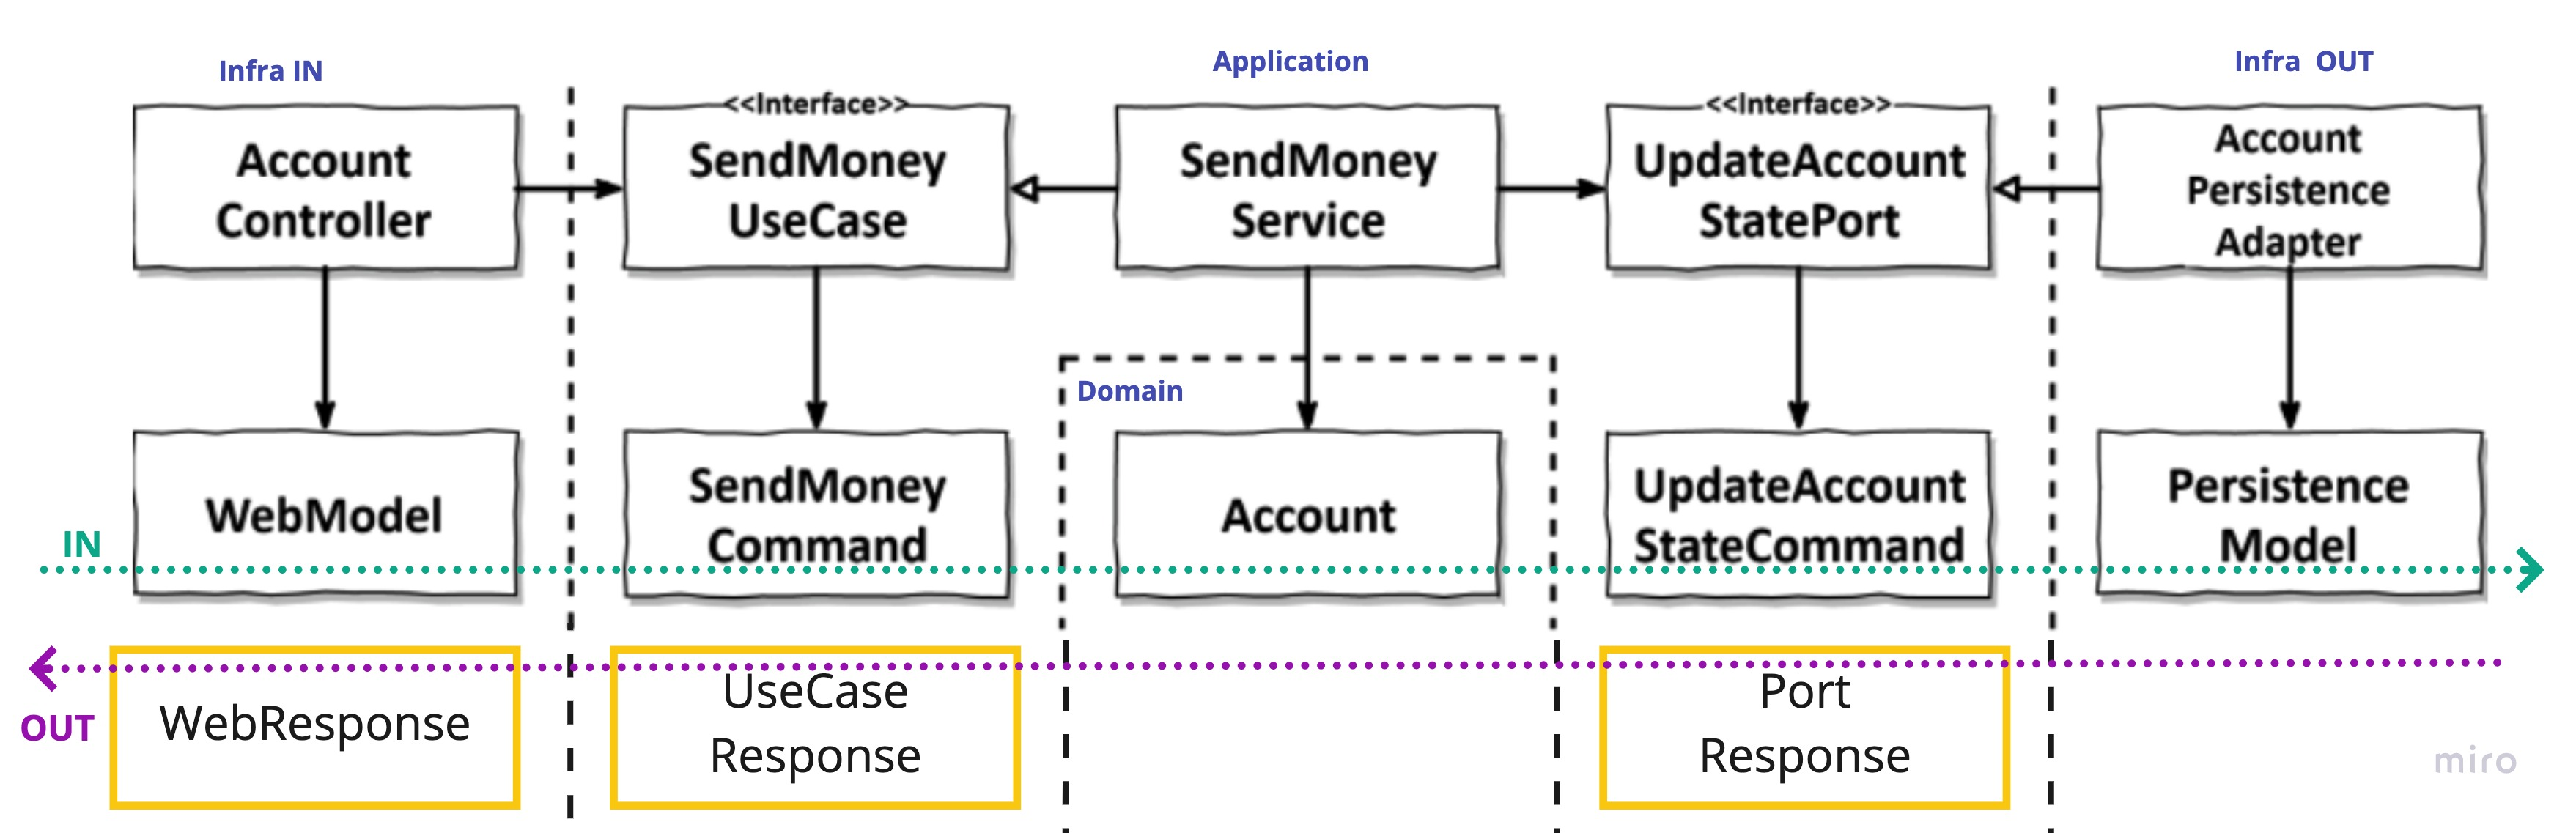
\includegraphics[height=0.2\textheight]{./part/Ejecucion/Seguimiento/CreateTaskUseCase/img/PFM - GetHandMapping}
    \caption{CreateTaskUseCase folder Structure\cite{TomHombergs2019GYHD}}\label{fig:GetHandMapping}
\end{figure}

Claramente esto aumenta la burocracia y finalmente la opción que hemos tomado se puede ver en la figura\ref{fig:CreateTaskUseCaseMapping}

En rojo se han marcado los atajos que se han tomado, es decir, el mapeo que no se ha implementado. El objetivo es aislarse bien de los puertos de entrada, es decir el GRPC, y no tanto de los puertos de salida. ya que la persistencia está bien aislada mediante las interfaces. Dentro de los adaptadores se hará el trabajo de mappeo entre las entidades de dominio y los modelos de persistencia y se traducirá de nuevo a dominio para responder.

\begin{figure}[H]
    \centering
    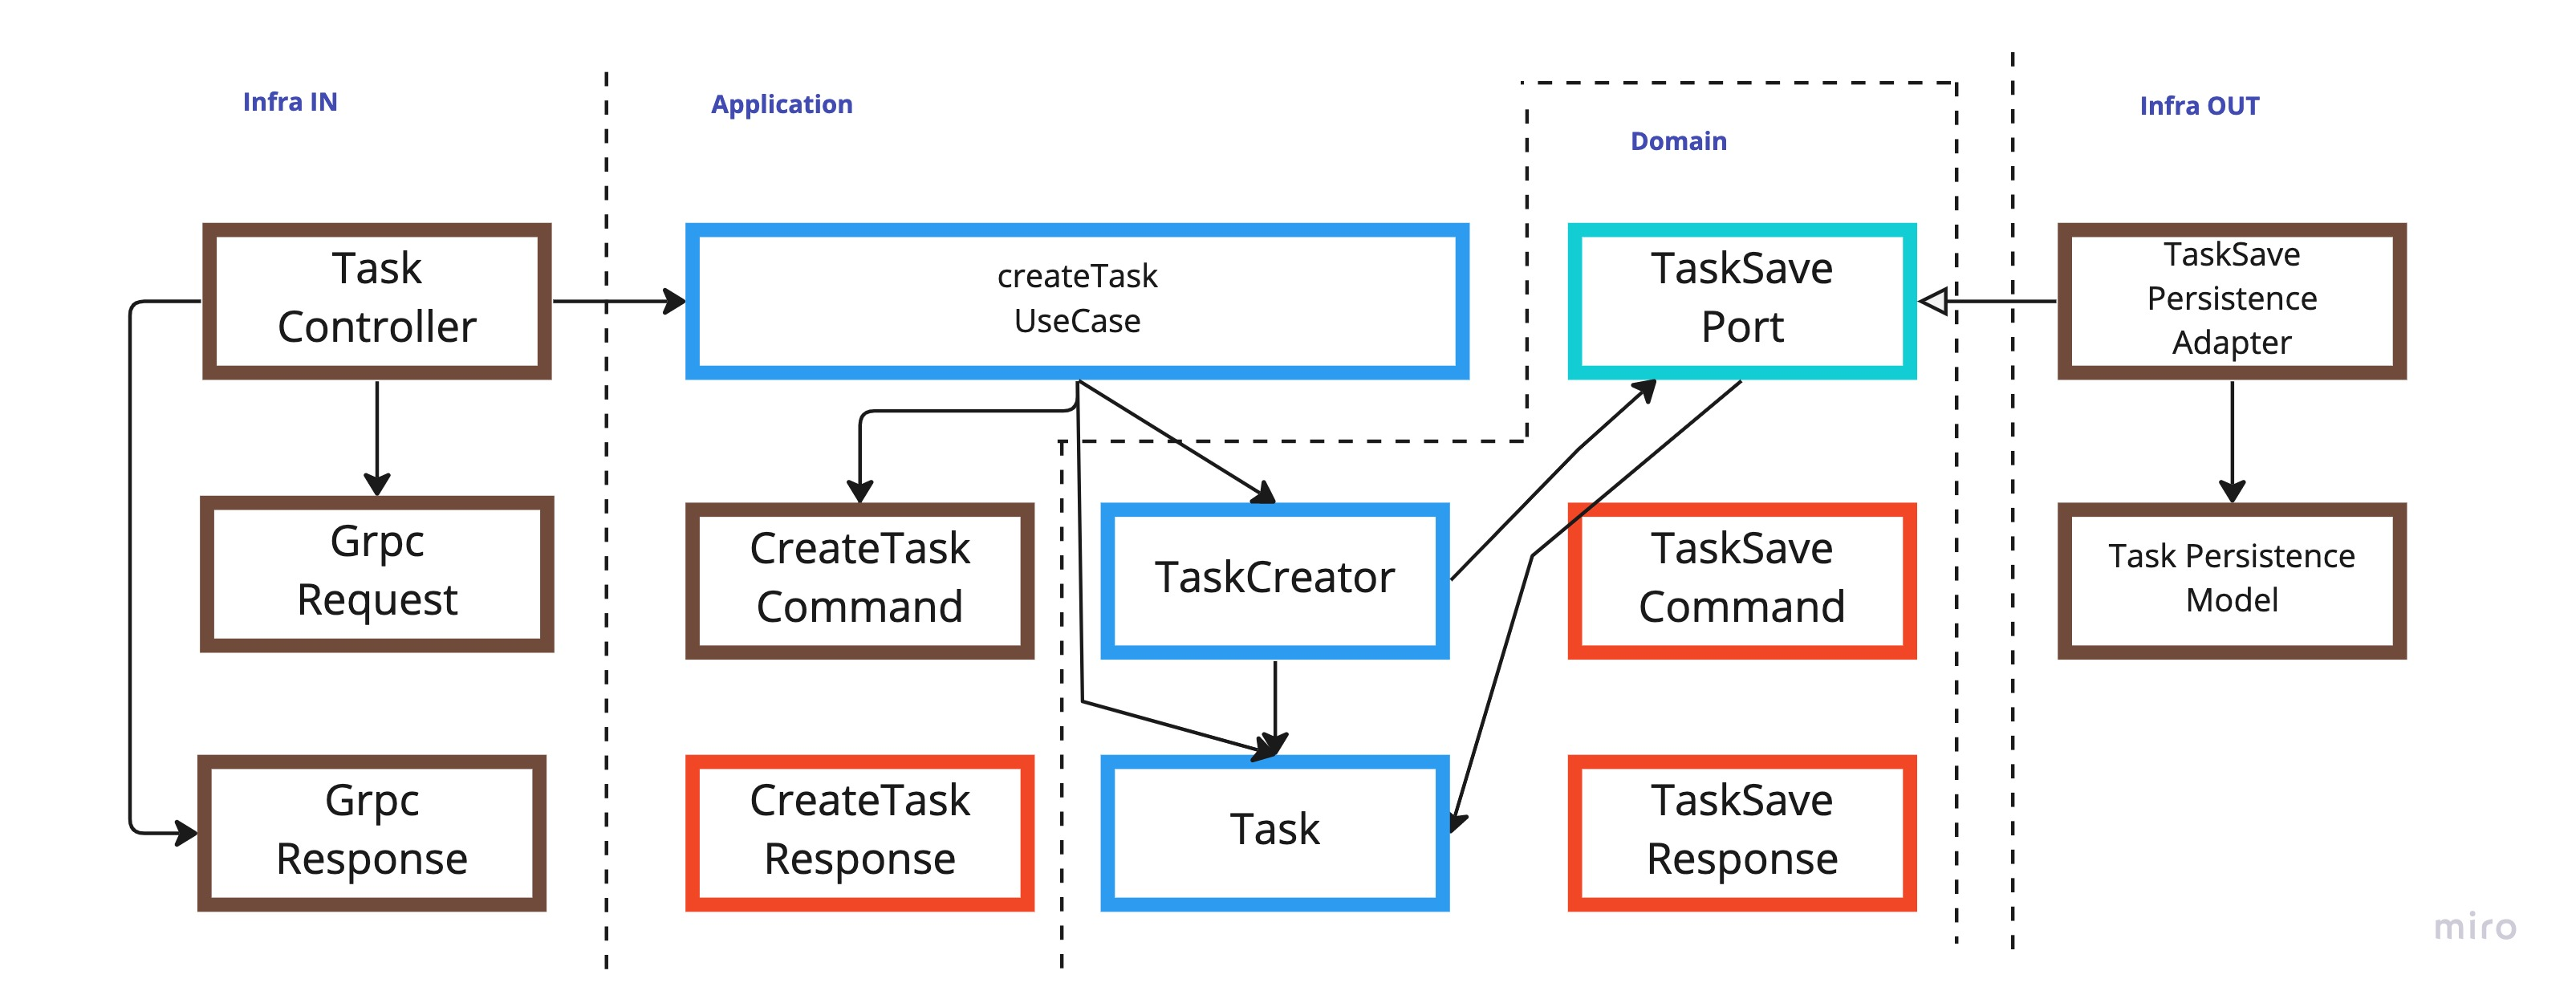
\includegraphics[height=0.2\textheight]{./part/Ejecucion/Seguimiento/CreateTaskUseCase/img/PFM - FinalMapping}
    \caption{CreateTaskUseCase folder Structure}\label{fig:CreateTaskUseCaseMapping}
\end{figure}

Ahora vamos a exponer el código final de este caso de uso, vamos a hacer referencia a:
\begin{itemize}
    \item TaskController \ref{fig:TaskControler}
    \item CreateTaskUseCase \ref{fig:CreateTaskUseCaseCode}
    \item Creator \ref{fig:Creator}
    \item SavePort \ref{fig:SavePort}
    \item PersistAdapter \ref{fig:SaveAdapter}
    \item DispatcherPort \ref{fig:DispatcherPort}
\end{itemize}

\begin{figure}[H]
    \centering
    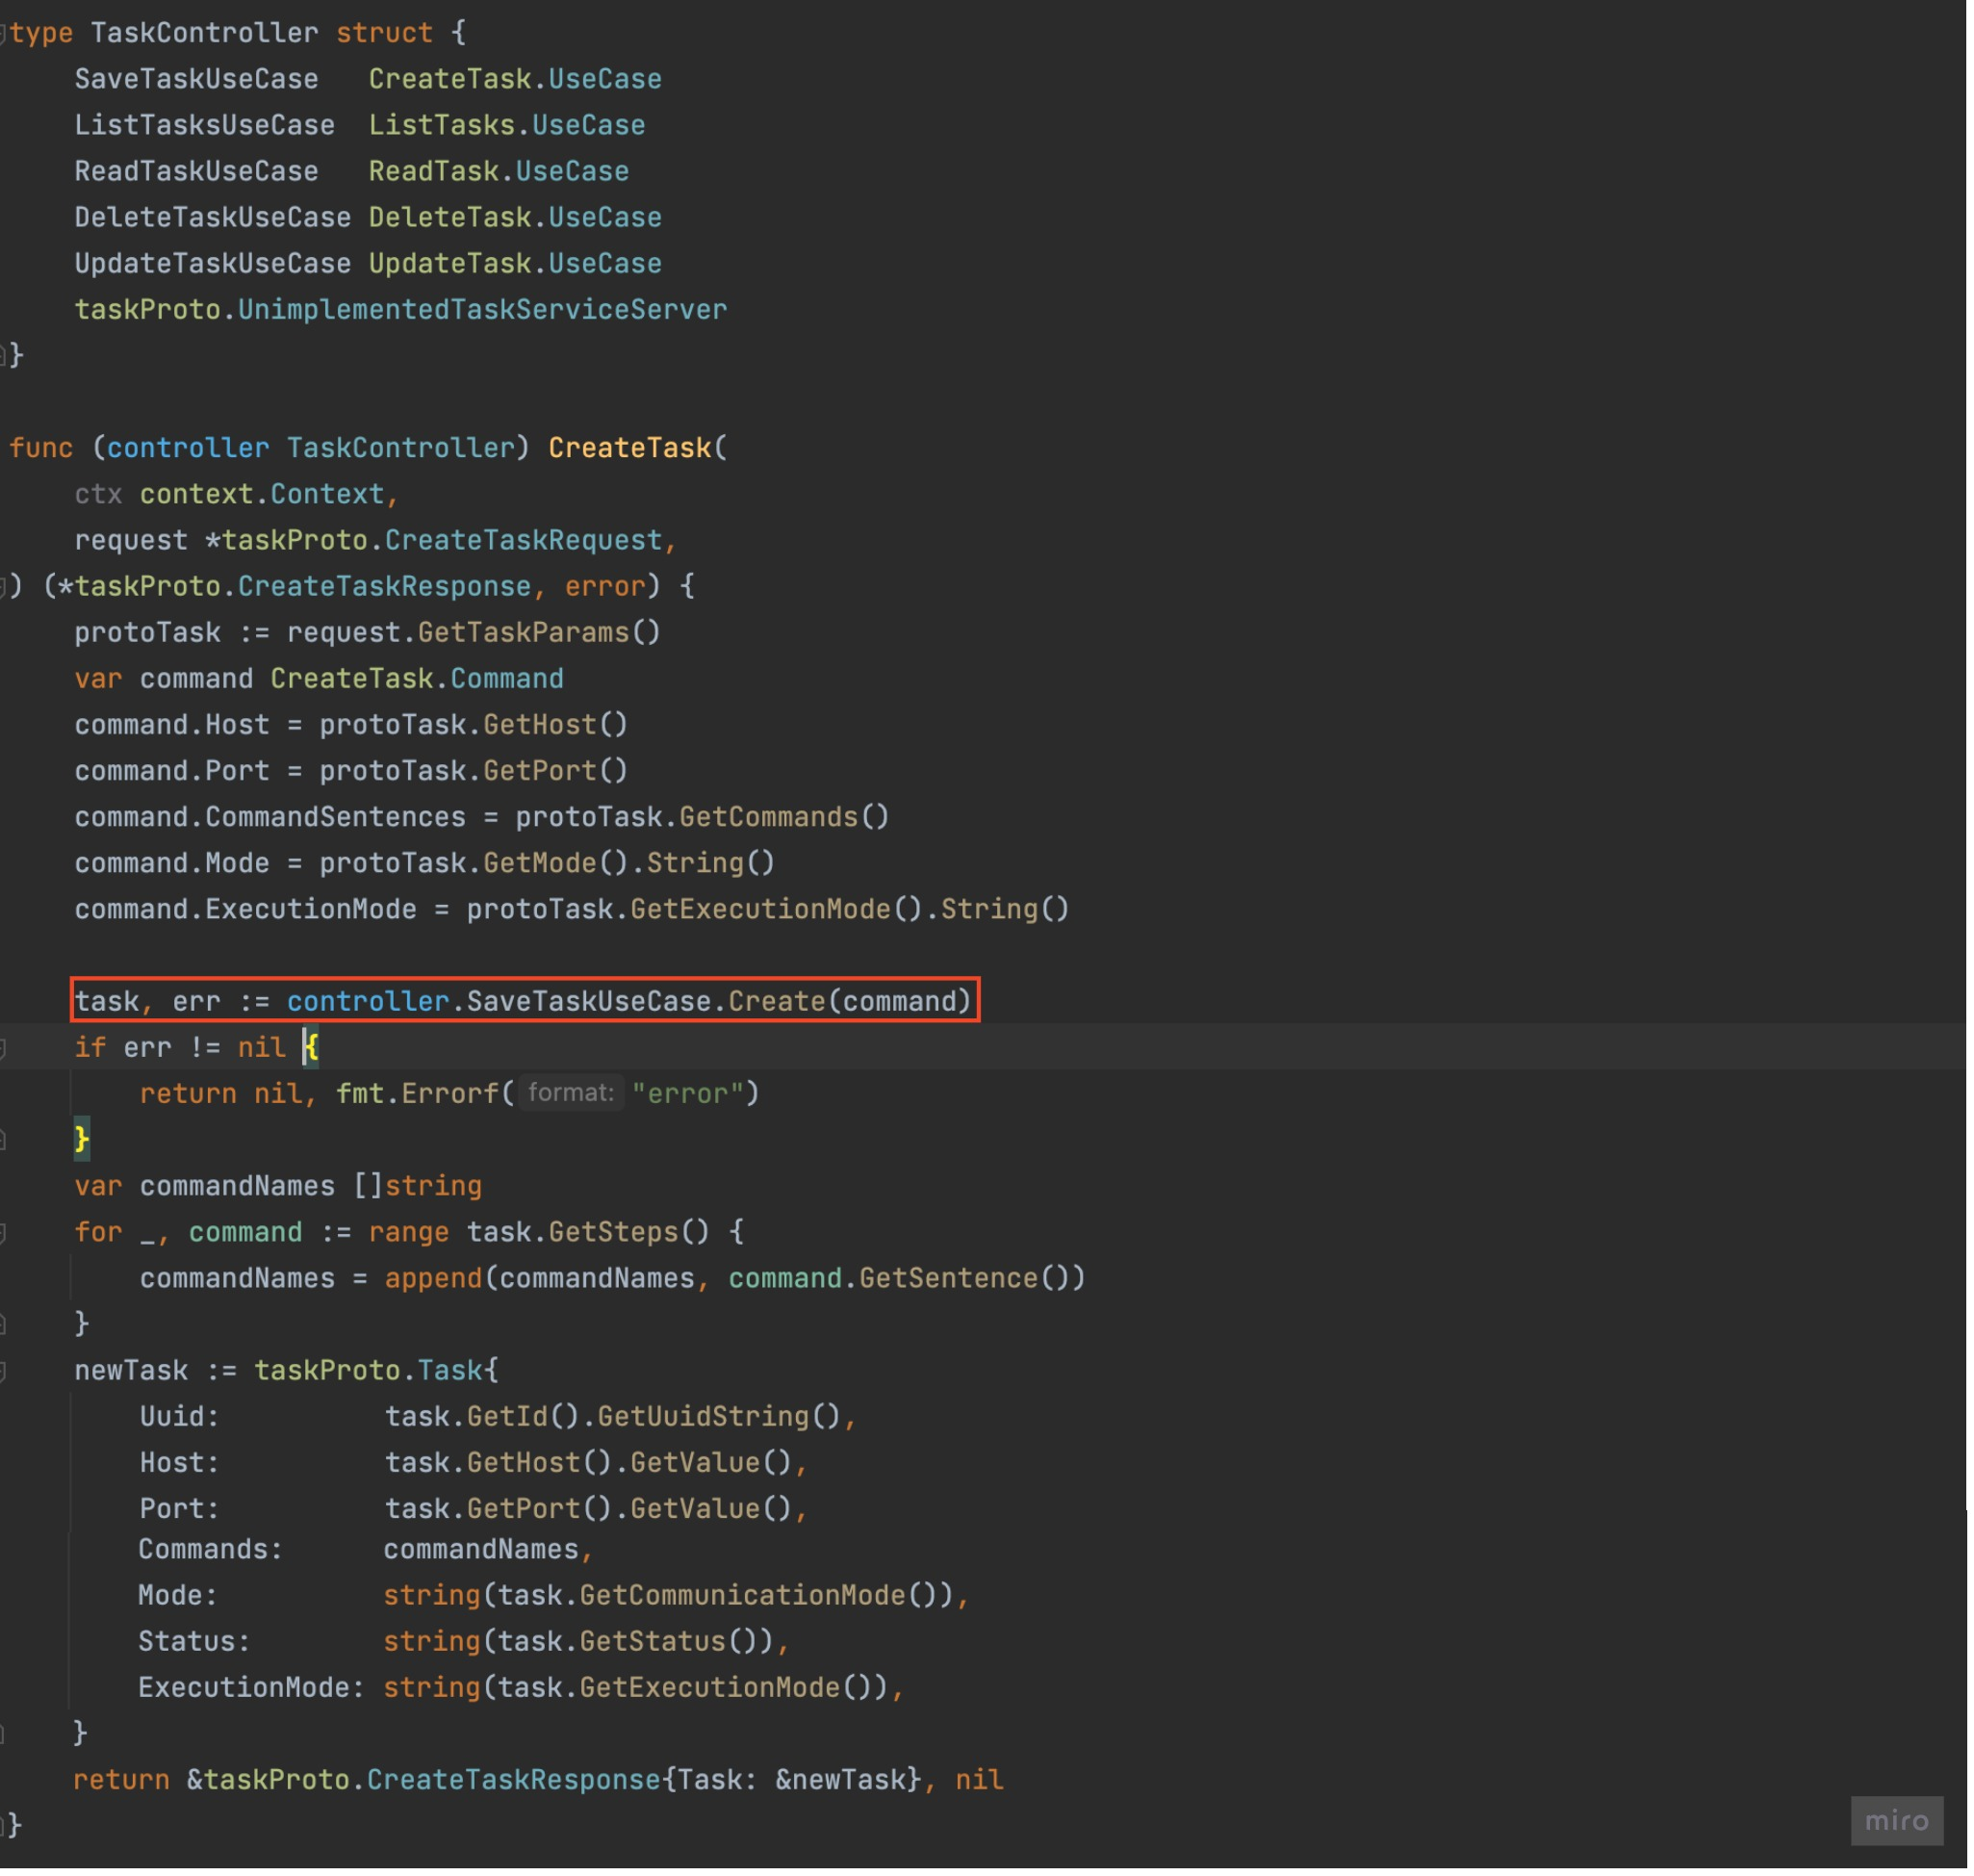
\includegraphics[height=0.5\textheight]{./part/Ejecucion/Seguimiento/CreateTaskUseCase/img/PFM - TaskController}
    \caption{TaskController.go}\label{fig:TaskControler}
\end{figure}

\begin{figure}[H]
    \centering
    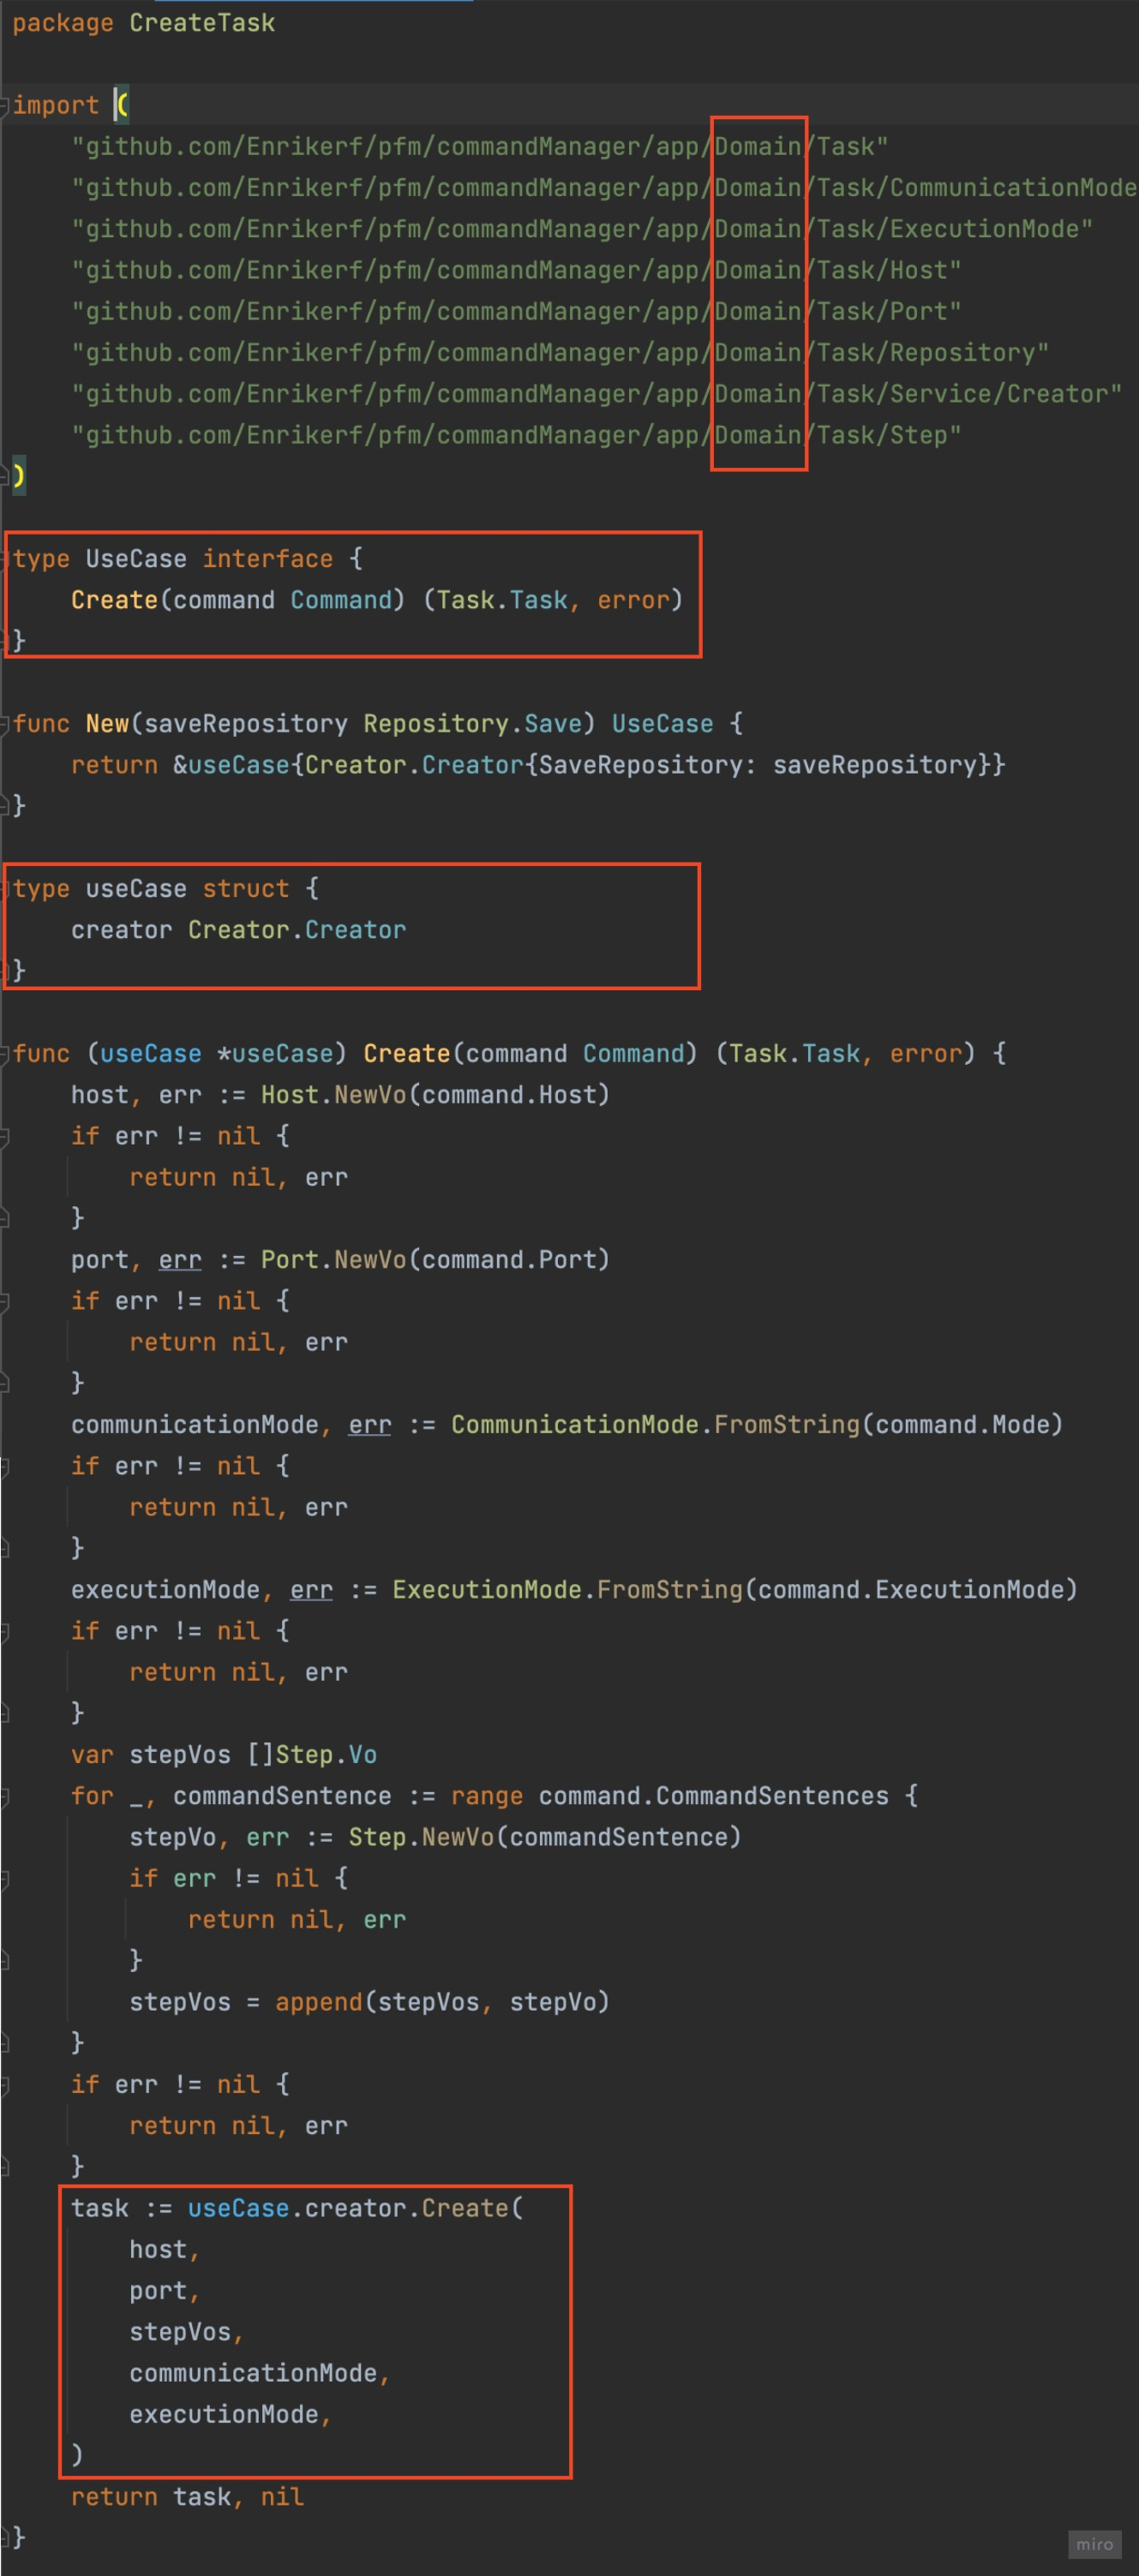
\includegraphics[height=0.5\textheight]{./part/Ejecucion/Seguimiento/CreateTaskUseCase/img/PFM - CreateTaskUseCaseCode}
    \caption{CreateTaskUseCaseCode.go}\label{fig:CreateTaskUseCaseCode}
\end{figure}

\begin{figure}[H]
    \centering
    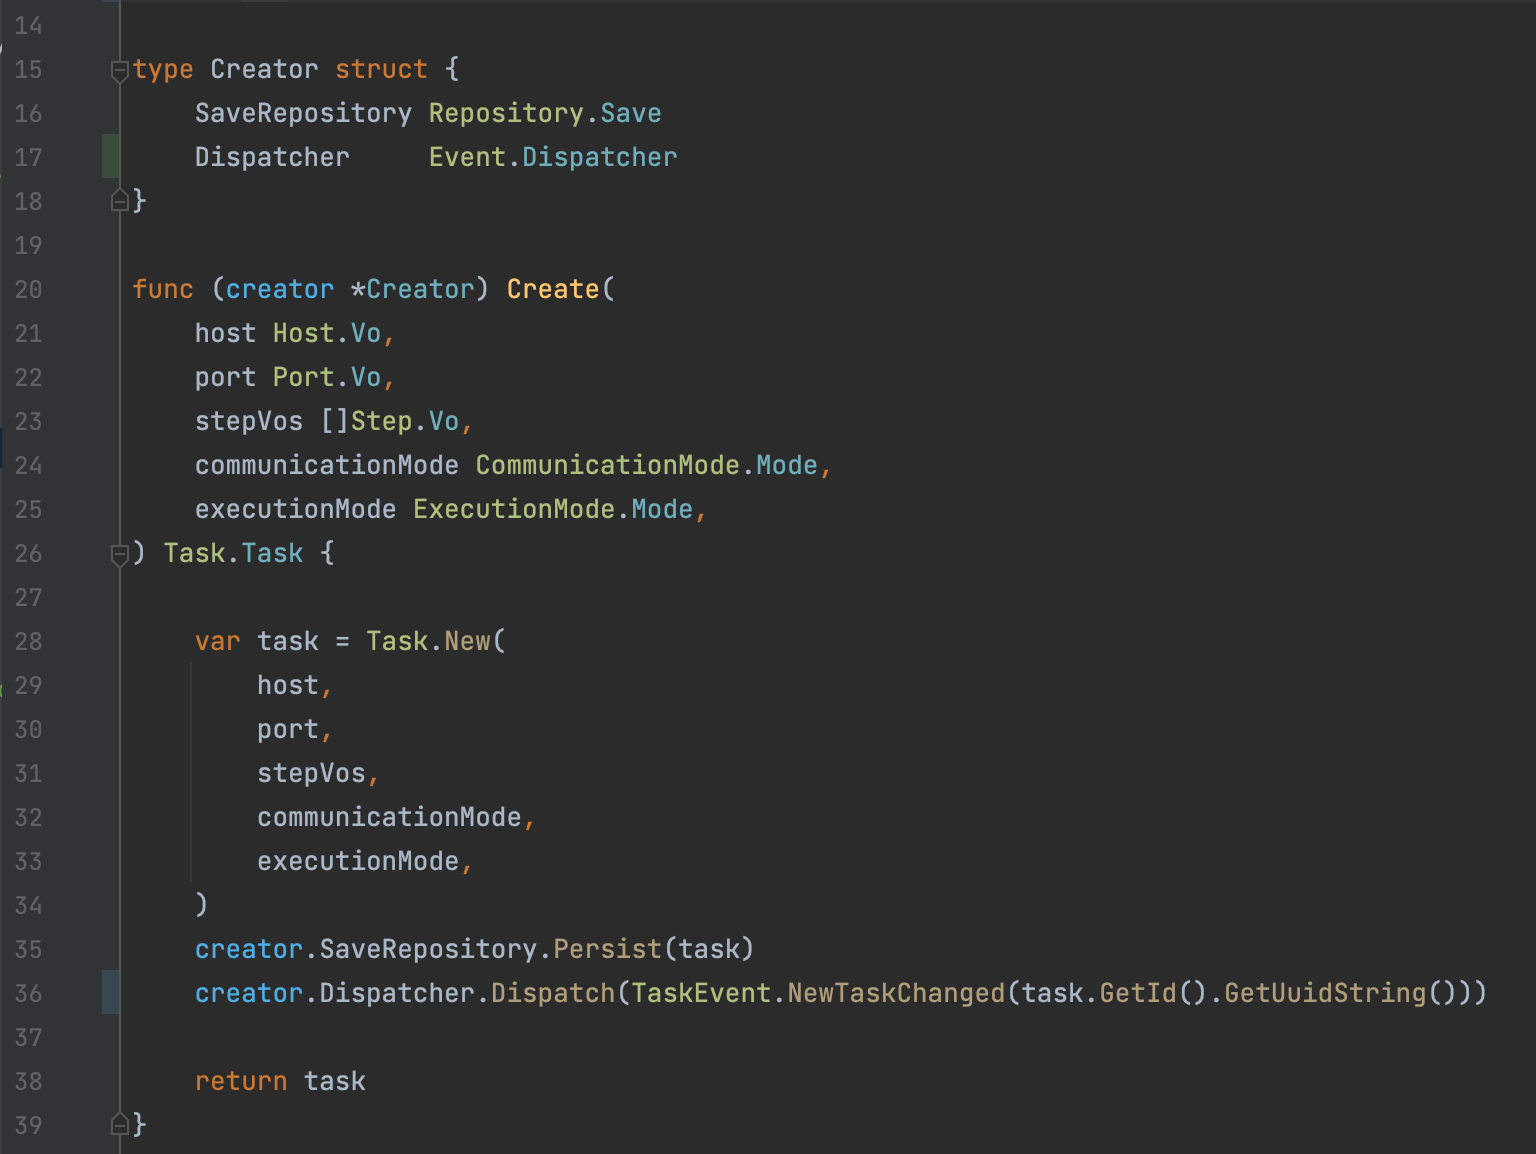
\includegraphics[height=0.5\textheight]{./part/Ejecucion/Seguimiento/CreateTaskUseCase/img/PFM - creator}
    \caption{Creator.go}\label{fig:Creator}
\end{figure}

\begin{figure}[H]
    \centering
    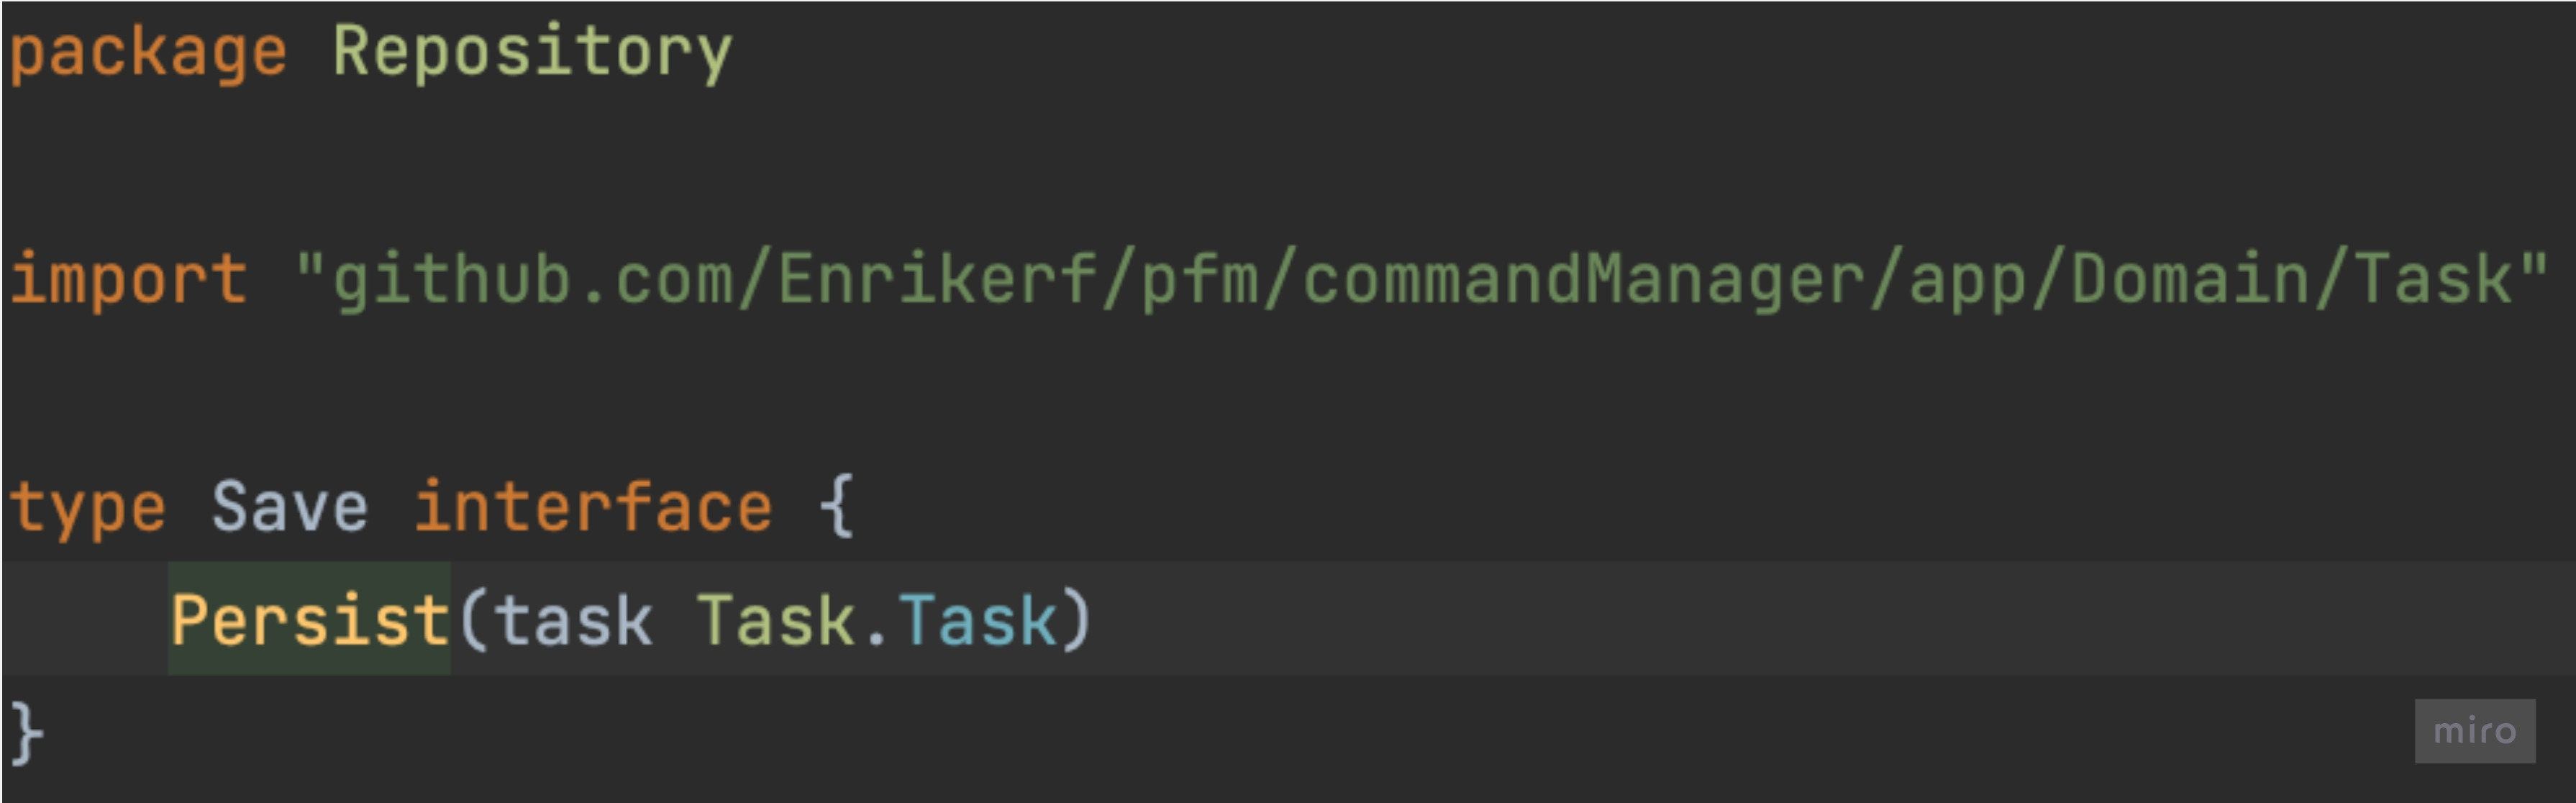
\includegraphics[height=0.2\textheight]{./part/Ejecucion/Seguimiento/CreateTaskUseCase/img/PFM - SavePort}
    \caption{Creator.go}\label{fig:SavePort}
\end{figure}

\begin{figure}[H]
    \centering
    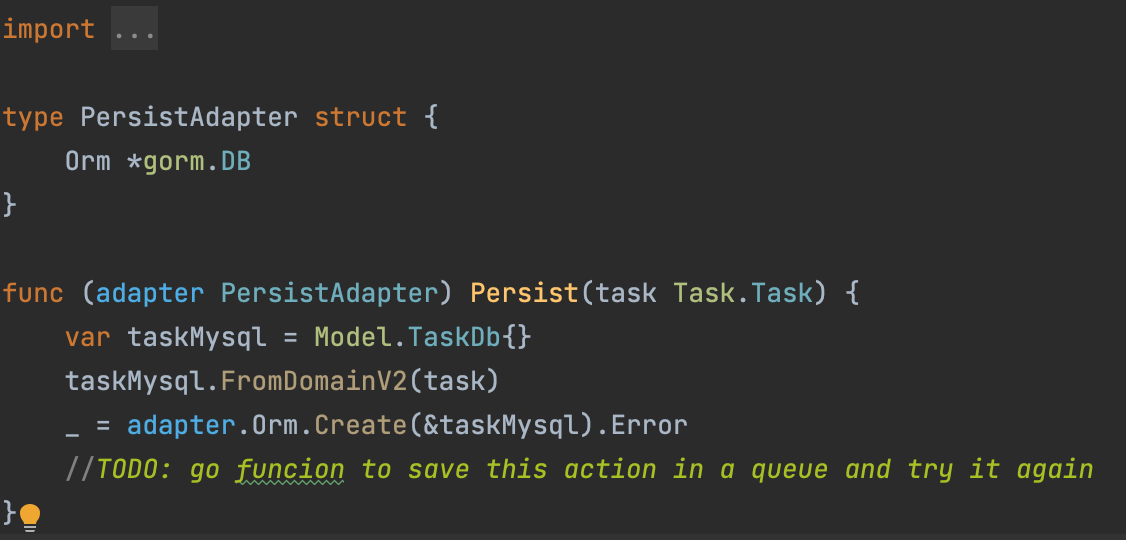
\includegraphics[height=0.2\textheight]{./part/Ejecucion/Seguimiento/CreateTaskUseCase/img/PFM - SaveAdapter}
    \caption{Creator.go}\label{fig:SaveAdapter}
\end{figure}

\begin{figure}[H]
    \centering
    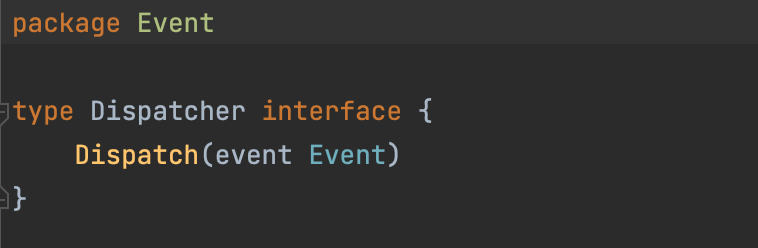
\includegraphics[height=0.2\textheight]{./part/Ejecucion/Seguimiento/CreateTaskUseCase/img/PFM - Dispatcher}
    \caption{Creator.go}\label{fig:DispatcherPort}
\end{figure}
\subsubsection{TaskEventHandler}
    

El adaptador de salida \textit{Dispatcher}~\cref{lst:DispatcherAdapter} es a su vez un elemento que actuará como adaptador de entrada.
Ejecutará el caso de uso \textit{TaskEventHandlerUseCase}~\cref{lst:TaskEventHandlerUseCase} cuando el evento lanzado sea de tipo .\textit{TaskCreated}
Podemos ver en~\cref{lst:DispatcherAdapter} que el gestor de eventos está preparado para añadir más eventos y gestionar otros casos de uso en consecuencia.

\textit{TaskEventHandlerUseCase}~\cref{lst:TaskEventHandlerUseCase} Habilitará el \textit{Looper}~\cref{lst:Looper} si la tarea creada es de tipo AUTOMATIC y el status es PENDING\@.
El servicio de Dominio \textit{Looper} buscará todas las tareas automáticas pendientes y las ejecutará de forma asíncrona.

En el servicio \textit{Looper}~\cref{lst:Looper}, señalado en rojo está el bloque de gestión de las operaciones asíncronas.
Por cada tarea se crea un hilo de ejecución paralelo.
Cuando todos los hilos terminan el comando \textit{wg.Wait()} desbloquea la ejecución del \textit{Looper}.


\phantom{blank}
\vspace{5mm}
\hrule
\begin{lstlisting}[language=Go,caption={DispatcherAdapter.go},breaklines=true,label={lst:DispatcherAdapter}]
package EventDispatcherAdapter

import (
	"github.com/Enrikerf/pfm/commandManager/app/Application/Port/In/Task/TaskEventHandler"
	"github.com/Enrikerf/pfm/commandManager/app/Domain/Event"
	TaskEvent "github.com/Enrikerf/pfm/commandManager/app/Domain/Task/Event"
)

type EventDispatcherAdapter interface {
	Dispatch(event Event.Event)
}

type eventDispatcherAdapter struct {
	taskEventHandler TaskEventHandler.UseCase
}

func New(
	taskEventHandler TaskEventHandler.UseCase,
) EventDispatcherAdapter {
	self := &eventDispatcherAdapter{
		taskEventHandler,
	}
	return self
}

func (e *eventDispatcherAdapter) Dispatch(event Event.Event) {
	switch event.GetName() {
	case TaskEvent.TaskCreatedEventName:
		go e.taskEventHandler.Handle(event)
	}
}


\end{lstlisting}
\hrule


El adaptador de salida \textit{Dispatcher}~\cref{lst:DispatcherAdapter} es a su vez un elemento que actuará como adaptador de entrada.
Ejecutará el caso de uso \textit{TaskEventHandlerUseCase}~\cref{lst:TaskEventHandlerUseCase} cuando el evento lanzado sea de tipo .\textit{TaskCreated}
Podemos ver en~\cref{lst:DispatcherAdapter} que el gestor de eventos está preparado para añadir más eventos y gestionar otros casos de uso en consecuencia.

\textit{TaskEventHandlerUseCase}~\cref{lst:TaskEventHandlerUseCase} Habilitará el \textit{Looper}~\cref{lst:Looper} si la tarea creada es de tipo AUTOMATIC y el status es PENDING\@.
El servicio de Dominio \textit{Looper} buscará todas las tareas automáticas pendientes y las ejecutará de forma asíncrona.

En el servicio \textit{Looper}~\cref{lst:Looper}, señalado en rojo está el bloque de gestión de las operaciones asíncronas.
Por cada tarea se crea un hilo de ejecución paralelo.
Cuando todos los hilos terminan el comando \textit{wg.Wait()} desbloquea la ejecución del \textit{Looper}.


\phantom{blank}
\vspace{5mm}
\hrule
\begin{lstlisting}[language=Go,caption={DispatcherAdapter.go},breaklines=true,label={lst:DispatcherAdapter}]
package EventDispatcherAdapter

import (
	"github.com/Enrikerf/pfm/commandManager/app/Application/Port/In/Task/TaskEventHandler"
	"github.com/Enrikerf/pfm/commandManager/app/Domain/Event"
	TaskEvent "github.com/Enrikerf/pfm/commandManager/app/Domain/Task/Event"
)

type EventDispatcherAdapter interface {
	Dispatch(event Event.Event)
}

type eventDispatcherAdapter struct {
	taskEventHandler TaskEventHandler.UseCase
}

func New(
	taskEventHandler TaskEventHandler.UseCase,
) EventDispatcherAdapter {
	self := &eventDispatcherAdapter{
		taskEventHandler,
	}
	return self
}

func (e *eventDispatcherAdapter) Dispatch(event Event.Event) {
	switch event.GetName() {
	case TaskEvent.TaskCreatedEventName:
		go e.taskEventHandler.Handle(event)
	}
}


\end{lstlisting}
\hrule


El adaptador de salida \textit{Dispatcher}~\cref{lst:DispatcherAdapter} es a su vez un elemento que actuará como adaptador de entrada.
Ejecutará el caso de uso \textit{TaskEventHandlerUseCase}~\cref{lst:TaskEventHandlerUseCase} cuando el evento lanzado sea de tipo .\textit{TaskCreated}
Podemos ver en~\cref{lst:DispatcherAdapter} que el gestor de eventos está preparado para añadir más eventos y gestionar otros casos de uso en consecuencia.

\textit{TaskEventHandlerUseCase}~\cref{lst:TaskEventHandlerUseCase} Habilitará el \textit{Looper}~\cref{lst:Looper} si la tarea creada es de tipo AUTOMATIC y el status es PENDING\@.
El servicio de Dominio \textit{Looper} buscará todas las tareas automáticas pendientes y las ejecutará de forma asíncrona.

En el servicio \textit{Looper}~\cref{lst:Looper}, señalado en rojo está el bloque de gestión de las operaciones asíncronas.
Por cada tarea se crea un hilo de ejecución paralelo.
Cuando todos los hilos terminan el comando \textit{wg.Wait()} desbloquea la ejecución del \textit{Looper}.

\input{./part/Ejecucion/Seguimiento/TaskEventHandler/codes/EventDispatcherAdapter}
\input{./part/Ejecucion/Seguimiento/TaskEventHandler/codes/TaskEventHandlerUseCase}
\input{./part/Ejecucion/Seguimiento/TaskEventHandler/codes/Looper}


\phantom{blank}
\vspace{5mm}
\hrule
\begin{lstlisting}[language=Go,caption={Looper.go},breaklines=true,label={lst:Looper}]
package Looper

import (
	"fmt"
	"github.com/Enrikerf/pfm/commandManager/app/Domain/Communication/Repository"
	ResultRepository "github.com/Enrikerf/pfm/commandManager/app/Domain/Result/Repository"
	"github.com/Enrikerf/pfm/commandManager/app/Domain/Task"
	"github.com/Enrikerf/pfm/commandManager/app/Domain/Task/ExecutionMode"
	TaskRepository "github.com/Enrikerf/pfm/commandManager/app/Domain/Task/Repository"
	"github.com/Enrikerf/pfm/commandManager/app/Domain/Task/Status"
	"sync"
)

var once sync.Once
var instance Looper

type Looper interface {
	IsEnabled() bool
	Enable()
}

func NewLooper(
	communicateRepository Repository.Communicate,
	findTasksByRepository TaskRepository.FindBy,
	saveTaskRepository TaskRepository.Save,
	saveBatchRepository ResultRepository.SaveBatch,
	saveResultRepository ResultRepository.Save,
) Looper {
	once.Do(func() {
		instance = &looper{
			communicateRepository: communicateRepository,
			findTasksByRepository: findTasksByRepository,
			saveTaskRepository:    saveTaskRepository,
			saveBatchRepository:   saveBatchRepository,
			saveResultRepository:  saveResultRepository,
			isLoopEnabled:         make(chan bool, 1),
		}
	})
	return instance
}

type looper struct {
	communicateRepository Repository.Communicate
	findTasksByRepository TaskRepository.FindBy
	saveTaskRepository    TaskRepository.Save
	saveBatchRepository   ResultRepository.SaveBatch
	saveResultRepository  ResultRepository.Save
	isLoopEnabled         chan bool
}

func (l *looper) IsEnabled() bool {
	return len(l.isLoopEnabled) != 0
}

func (l *looper) Enable() {
	l.isLoopEnabled <- true
	go l.loop()
}

func (l *looper) loop() {
	for l.IsEnabled() {
		tasks, err := l.findTasksByRepository.FindBy(map[string]interface{}{
			"status":         Status.Pending,
			"execution_mode": ExecutionMode.Automatic,
		})
		if err != nil {
			fmt.Printf(err.Error())
			l.stopLoop()
			return
		}
		if len(tasks) < 1 {
			l.stopLoop()
			return
		}
		<@\textcolor{red}{//---async waiting block---}@>
		var wg sync.WaitGroup
		for index := range tasks {
			wg.Add(1)
			go l.executeTask(&wg, tasks[index])
		}
		wg.Wait()
		<@\textcolor{red}{//------}@>
	}
}

func (l *looper) executeTask(wg *sync.WaitGroup, task Task.Task) {
	defer wg.Done()
	task.SetStatus(Status.New(Status.Running))
	l.saveTaskRepository.Persist(task)
	resultBatch := l.communicateRepository.Communicate(task)
	l.saveBatchRepository.Persist(resultBatch)
	task.SetStatus(Status.New(Status.Done))
	l.saveTaskRepository.Persist(task)
}

func (l *looper) stopLoop() {
	if len(l.isLoopEnabled) > 0 {
		fmt.Println("loop stopped")
		<-l.isLoopEnabled
	} else {
		fmt.Println("trying to stop loop but is not running")
	}
}


\end{lstlisting}
\hrule


\phantom{blank}
\vspace{5mm}
\hrule
\begin{lstlisting}[language=Go,caption={Looper.go},breaklines=true,label={lst:Looper}]
package Looper

import (
	"fmt"
	"github.com/Enrikerf/pfm/commandManager/app/Domain/Communication/Repository"
	ResultRepository "github.com/Enrikerf/pfm/commandManager/app/Domain/Result/Repository"
	"github.com/Enrikerf/pfm/commandManager/app/Domain/Task"
	"github.com/Enrikerf/pfm/commandManager/app/Domain/Task/ExecutionMode"
	TaskRepository "github.com/Enrikerf/pfm/commandManager/app/Domain/Task/Repository"
	"github.com/Enrikerf/pfm/commandManager/app/Domain/Task/Status"
	"sync"
)

var once sync.Once
var instance Looper

type Looper interface {
	IsEnabled() bool
	Enable()
}

func NewLooper(
	communicateRepository Repository.Communicate,
	findTasksByRepository TaskRepository.FindBy,
	saveTaskRepository TaskRepository.Save,
	saveBatchRepository ResultRepository.SaveBatch,
	saveResultRepository ResultRepository.Save,
) Looper {
	once.Do(func() {
		instance = &looper{
			communicateRepository: communicateRepository,
			findTasksByRepository: findTasksByRepository,
			saveTaskRepository:    saveTaskRepository,
			saveBatchRepository:   saveBatchRepository,
			saveResultRepository:  saveResultRepository,
			isLoopEnabled:         make(chan bool, 1),
		}
	})
	return instance
}

type looper struct {
	communicateRepository Repository.Communicate
	findTasksByRepository TaskRepository.FindBy
	saveTaskRepository    TaskRepository.Save
	saveBatchRepository   ResultRepository.SaveBatch
	saveResultRepository  ResultRepository.Save
	isLoopEnabled         chan bool
}

func (l *looper) IsEnabled() bool {
	return len(l.isLoopEnabled) != 0
}

func (l *looper) Enable() {
	l.isLoopEnabled <- true
	go l.loop()
}

func (l *looper) loop() {
	for l.IsEnabled() {
		tasks, err := l.findTasksByRepository.FindBy(map[string]interface{}{
			"status":         Status.Pending,
			"execution_mode": ExecutionMode.Automatic,
		})
		if err != nil {
			fmt.Printf(err.Error())
			l.stopLoop()
			return
		}
		if len(tasks) < 1 {
			l.stopLoop()
			return
		}
		<@\textcolor{red}{//---async waiting block---}@>
		var wg sync.WaitGroup
		for index := range tasks {
			wg.Add(1)
			go l.executeTask(&wg, tasks[index])
		}
		wg.Wait()
		<@\textcolor{red}{//------}@>
	}
}

func (l *looper) executeTask(wg *sync.WaitGroup, task Task.Task) {
	defer wg.Done()
	task.SetStatus(Status.New(Status.Running))
	l.saveTaskRepository.Persist(task)
	resultBatch := l.communicateRepository.Communicate(task)
	l.saveBatchRepository.Persist(resultBatch)
	task.SetStatus(Status.New(Status.Done))
	l.saveTaskRepository.Persist(task)
}

func (l *looper) stopLoop() {
	if len(l.isLoopEnabled) > 0 {
		fmt.Println("loop stopped")
		<-l.isLoopEnabled
	} else {
		fmt.Println("trying to stop loop but is not running")
	}
}


\end{lstlisting}
\hrule

\subsubsection{PID Control}\label{subsubsec:pidControl}
    Control Algorithm:



Dentro del Dominio del controlador tendremos Un modelo de lo que significa para nosotros un encoder.
Podemos ver en la figura~\cref{fig:EncoderInterface} que es una interfaz que actua como puerto de salida hacia la implementación, el adaptador que contemplará el uso de una librería en golang para raspberry que permita la interacción de los pines de lectura con los que está conectado el encoder y realice las operaciones pertinentes para obtener la posición.
Todo esto no es responsabilidad del Dominio.
No nos atañe el dispositivo en el que se va a ejecutar la lógica de control a partir de este encoder.
Simplemente nos interesa que tenga una función de observación que llamaremos \textit{watchdog} de las lectura de dichos pines y una función a la que llamaremos para obtener la posición en el momento que deseemos saberlo \textit{getPosition} También atañe al dominio saber que hay que resetear los parámetros del encoder cuando interese y que hay que desactivar el hardware cuando se deje de utilizar para que no haya inconsistencias a la hora de volver a ejecutar el programa.


\begin{figure}[H]
    \centering
    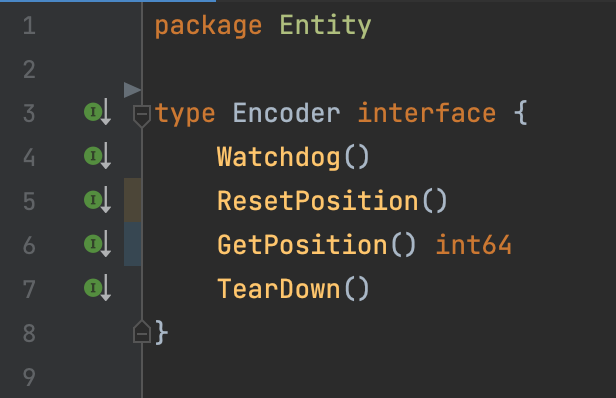
\includegraphics[height=0.2\textheight]{./part/Ejecucion/Seguimiento/PidControl/img/EncoderInterface}
    \caption{Encoder.go}\label{fig:EncoderInterface}
\end{figure}

Pasando a la implementación el punto de más relevancia se encuentra remarcado en rojo en la figura~\cref{fig:EncoderAdapter} donde podemos ver que cuando se ejecuta la función de \textit{watchdog} se ponen en marcha dos gorutines; una para vigilar cada lectura de los dos pines del Encoder.

Se queda en un bucle infinito la primera sentencia de dicho bucle es quedarse bloqueado hasta que haya un cambio en el pin de lectura, ya sea de 0 a 1 o de 1 a 0.
Si esto ocurre lo primero que hace es bloquear todas las demas gorutines porque va a hacer cambios en memoria de forma atómica, escribe la información de dicha lectura en un array de lecturas y desbloquea las gorutines, se termina y vuelve a esperar.

Independientemente, el watchdog, una vez lanzadas las gorutines de lectura se queda en bucle infinito que lo que hace es bloquear las gorutinas.
Extraer un elemento del array de lecturas y procesarlo.

Tal y como están diseñadas la gorutines, se van encolando y esperan su momento en la CPU para ejecutarse.
si hay bloqueos también esperan su turno.
De esta forma supongamos que el procesado de una lectura tardara más de la cuenta.
Se irían encolando las gorutines a la espera de poder añadirse en el array de lecturas, pero no se perderían.
De esta forma Se consigue leer exactamente los 360 pulsos por vuelta del encoder sin perder ninguno.

\begin{figure}[H]
    \centering
    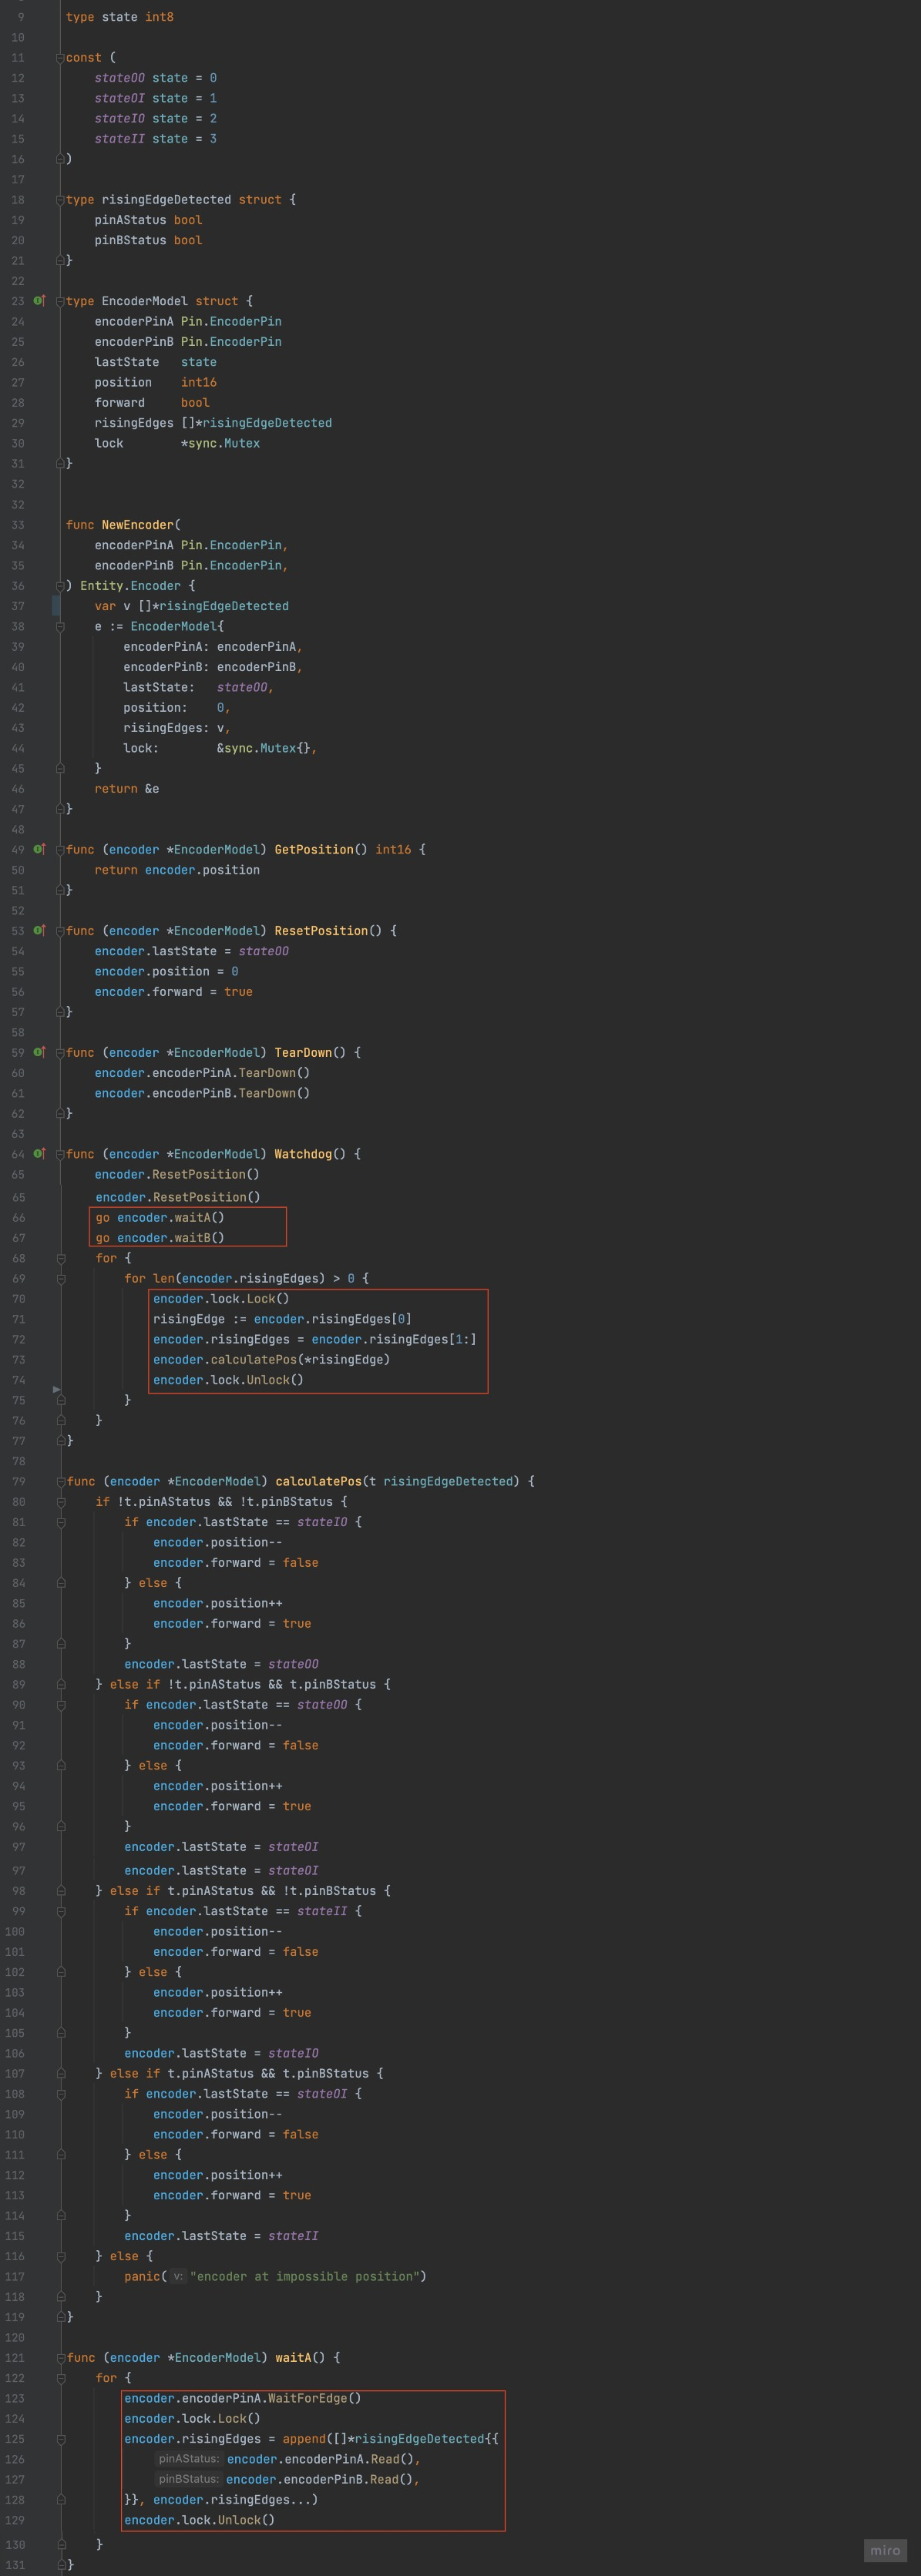
\includegraphics[height=0.95\textheight]{./part/Ejecucion/Seguimiento/PidControl/img/PFM - Encoder}
    \caption{EncoderAdapter.go}\label{fig:EncoderAdapter}
\end{figure}
\subsubsection{Testing}
    Para el caso de uso de Create task siguiendo\ref{par:testing}

Primero tenemos que localizar los factores o variables independientes

\begin{itemize}
    \item Host
    \item Port
    \item CommunicationMode
    \item ExecutionMode
    \item Steps
\end{itemize}

luego las clases de equivalencia:

\begin{itemize}
    \item Host: valid/invalid
    \item Port: valid/invalid
    \item CommunicationMode: valid/invalid
    \item ExecutionMode: valid/invalid
    \item Steps: valid/invalid
\end{itemize}

Cabe reseñar que el trabajo de buscar las clases de equivalencia no es trivial. por ejemplo, en el caso de steps que es un array podría haberse pensado que se necesita probar con varios elementos en el array, validos e invalidos, pero no tiene sentido porque la lógica debe contemplar únicamente

o por ejemplo en el caso de Host o Port que tiene validaciones. podría pensarse que debería ponerse a prueba con varios casos que den invalido, al ser un string libre y que ponga a prueba dicha validación, pero estamos en el caso de uso, eso será responsabilidad del test unitario de Host y Port. para la lógica que nos atañe en este test lo único que importa es qué sucedera en el caso que sea válido o invalido.

En un ejemplo tan trivial puede llevar a subestimar el ejercicio de entender el alcance de la prueba y la correcta selección de las clases de equivalencia, pero es de suma importancia.

Bien pues con estas clases de equivalencia las posibilidades son \[ 2^5 = 32 \] casos con el método de pares se reduce a 6 y los pares posibles son 41

las combinaciones posibles son:

\begin{table}[H]
    \small
    \begin{tabular}{cccccc}
        \textbf{}   & \textbf{host} & \textbf{port} & \textbf{communicationMode} & \textbf{executionMode} & \textbf{sentences} \\
        \textbf{1}  & valid         & valid         & valid                      & valid                  & valid              \\
        \textbf{2}  & valid         & valid         & valid                      & valid                  & invalid            \\
        \textbf{3}  & valid         & valid         & valid                      & invalid                & valid              \\
        \textbf{4}  & valid         & valid         & valid                      & invalid                & invalid            \\
        \textbf{5}  & valid         & valid         & invalid                    & valid                  & valid              \\
        \textbf{6}  & valid         & valid         & invalid                    & valid                  & invalid            \\
        \textbf{7}  & valid         & valid         & invalid                    & invalid                & valid              \\
        \textbf{8}  & valid         & valid         & invalid                    & invalid                & invalid            \\
        \textbf{9}  & valid         & invalid       & valid                      & valid                  & valid              \\
        \textbf{10} & valid         & invalid       & valid                      & valid                  & invalid            \\
        \textbf{11} & valid         & invalid       & valid                      & invalid                & valid              \\
        \textbf{12} & valid         & invalid       & valid                      & invalid                & invalid            \\
        \textbf{13} & valid         & invalid       & invalid                    & valid                  & valid              \\
        \textbf{14} & valid         & invalid       & invalid                    & valid                  & invalid            \\
        \textbf{15} & valid         & invalid       & invalid                    & invalid                & valid              \\
        \textbf{16} & valid         & invalid       & invalid                    & invalid                & invalid            \\
        \textbf{17} & invalid       & valid         & valid                      & valid                  & valid              \\
        \textbf{18} & invalid       & valid         & valid                      & valid                  & invalid            \\
        \textbf{19} & invalid       & valid         & valid                      & invalid                & valid              \\
        \textbf{20} & invalid       & valid         & valid                      & invalid                & invalid            \\
        \textbf{21} & invalid       & valid         & invalid                    & valid                  & valid              \\
        \textbf{22} & invalid       & valid         & invalid                    & valid                  & invalid            \\
        \textbf{23} & invalid       & valid         & invalid                    & invalid                & valid              \\
        \textbf{24} & invalid       & valid         & invalid                    & invalid                & invalid            \\
        \textbf{25} & invalid       & invalid       & valid                      & valid                  & valid              \\
        \textbf{26} & invalid       & invalid       & valid                      & valid                  & invalid            \\
        \textbf{27} & invalid       & invalid       & valid                      & invalid                & valid              \\
        \textbf{28} & invalid       & invalid       & valid                      & invalid                & invalid            \\
        \textbf{29} & invalid       & invalid       & invalid                    & valid                  & valid              \\
        \textbf{30} & invalid       & invalid       & invalid                    & valid                  & invalid            \\
        \textbf{31} & invalid       & invalid       & invalid                    & invalid                & valid              \\
        \textbf{32} & invalid       & invalid       & invalid                    & invalid                & invalid
    \end{tabular}
    \caption{tab:table2}\label{tab:table2}
\end{table}

y los pares son

\begin{table}[H]
    \small
    \begin{tabular}{llll}
        \textbf{var1}          & \textbf{var2}     & \textbf{value1} & \textbf{value2} \\
        \textbf{host}          & port              & valid           & valid           \\
        \textbf{host}          & port              & valid           & notValid        \\
        \textbf{host}          & port              & notValid        & valid           \\
        \textbf{host}          & port              & notValid        & notValid        \\
        \textbf{host}          & executionMode     & valid           & valid           \\
        \textbf{host}          & executionMode     & valid           & notValid        \\
        \textbf{host}          & executionMode     & notValid        & valid           \\
        \textbf{host}          & executionMode     & notValid        & notValid        \\
        \textbf{host}          & communicationMode & valid           & valid           \\
        \textbf{host}          & communicationMode & valid           & notValid        \\
        \textbf{host}          & communicationMode & notValid        & valid           \\
        \textbf{host}          & communicationMode & notValid        & notValid        \\
        \textbf{host}          & steps             & valid           & valid           \\
        \textbf{host}          & steps             & valid           & notValid        \\
        \textbf{host}          & steps             & notValid        & valid           \\
        \textbf{host}          & steps             & notValid        & notValid        \\
        \textbf{port}          & executionMode     & valid           & valid           \\
        \textbf{port}          & executionMode     & valid           & notValid        \\
        \textbf{port}          & executionMode     & notValid        & valid           \\
        \textbf{port}          & executionMode     & notValid        & notValid        \\
        \textbf{port}          & communicationMode & valid           & valid           \\
        \textbf{port}          & communicationMode & valid           & notValid        \\
        \textbf{port}          & communicationMode & notValid        & valid           \\
        \textbf{port}          & communicationMode & notValid        & notValid        \\
        \textbf{port}          & steps             & valid           & valid           \\
        \textbf{port}          & steps             & valid           & notValid        \\
        \textbf{port}          & steps             & notValid        & valid           \\
        \textbf{port}          & steps             & notValid        & notValid        \\
        \textbf{executionMode} & communicationMode & valid           & valid           \\
        \textbf{executionMode} & communicationMode & valid           & notValid        \\
        \textbf{executionMode} & communicationMode & notValid        & valid           \\
        \textbf{executionMode} & communicationMode & notValid        & notValid        \\
        executionMode          & steps             & valid           & valid           \\
        executionMode          & steps             & valid           & notValid        \\
        executionMode          & steps             & notValid        & valid           \\
        executionMode          & steps             & notValid        & notValid        \\
        communicationMode      & steps             & valid           & valid           \\
        communicationMode      & steps             & valid           & notValid        \\
        communicationMode      & steps             & notValid        & valid           \\
        communicationMode      & steps             & notValid        & notValid
    \end{tabular}
    \caption{tab:table3}\label{tab:table3}
\end{table}

El tests quedaría entonces como sale en la figura \ref{tab:createTaskPairWiseTest}

\begin{table}[H]
    \small
    \begin{tabular}{rllllll}
        case & host     & port     & ExeMode  & ComMode  & steps    & Expected Result        \\
        1    & valid    & valid    & valid    & valid    & valid    & OK                     \\
        2    & valid    & notValid & notValid & notValid & notValid & PortInvalidError       \\
        3    & notValid & valid    & notValid & valid    & notValid & HostInvalidError       \\
        4    & notValid & notValid & valid    & notValid & valid    & HostInvalidError       \\
        5    & ~valid   & valid    & valid    & notValid & notValid & CommunicationModeError \\
        6    & ~valid   & notValid & notValid & valid    & valid    & PortError
    \end{tabular}
    \caption{tab:createTaskPairWiseTest}\label{tab:createTaskPairWiseTest}
\end{table}

En la instaciación de una nueva Task tenemos los

Primero tenemos que localizar los factores o variables independientes

\begin{itemize}
    \item Number of steps
    \item execution Mode
    \item Communication Mode
\end{itemize}

luego las clases de equivalencia:

\begin{itemize}
    \item NSteps: 0,1,>2
    \item ExMod: Automatic, Manual
    \item ComMode: Server Stream,Client Stream, Bidirectional y Unary
\end{itemize}

tenemos entonces \[ 3*2*4 = 24 \] posibilidades pares obtenemos 27 al final queda reducidos a 13 casos. Vemos que la eficiencia en reducción de casos disminuye cuanto menos combinaciones hay. El diseño de los tests queda tal y como se ve en la tabla \ref{tab:taskTestPairwiseCases}

\begin{table}[H]
    \small
    \begin{tabular}{ccccl}
        \textbf{}   & \textbf{NSteps} & \textbf{ExeMod} & \textbf{ComMode} & \multicolumn{1}{c}{\textbf{Expected Result}}  \\
        \textbf{1}  & 0               & automatic       & serverStream     & NewTaskMustHaveAtLeastOneStepError            \\
        \textbf{2}  & 1               & automatic       & clientStream     & OK                                            \\
        \textbf{3}  & 1               & manual          & bidirectional    & OK                                            \\
        \textbf{4}  & 1               & automatic       & unary            & OK                                            \\
        \textbf{5}  & 1               & manual          & serverStream     & OK                                            \\
        \textbf{6}  & \textgreater{}2 & manual          & unary            & CommunicationModeCanOnlyHaveOneStepError      \\
        \textbf{7}  & \textgreater{}2 & automatic       & serverStream     & CommunicationModeCanOnlyHaveOneStepError      \\
        \textbf{8}  & \textgreater{}2 & manual          & clientStream     & OK                                            \\
        \textbf{9}  & \textgreater{}2 & automatic       & bidirectional    & ManualBidirectionalTaskOnlyCanHave2StepsError \\
        \textbf{10} & 0               & automatic       & clientStream     & TaskMustHaveAtLeastOneStepError               \\
        \textbf{11} & 0               & manual          & bidirectional    & TaskMustHaveAtLeastOneStepError               \\
        \textbf{12} & 0               & automatic       & unary            & TaskMustHaveAtLeastOneStepError               \\
        \textbf{13} & 0               & manual          & serverStream     & TaskMustHaveAtLeastOneStepError
    \end{tabular}
    \caption{tab:taskTestPairwiseCases}\label{tab:taskTestPairwiseCases}
\end{table}

Ahora vamos a ver cómo la arquitectura protege la calidad del sistema de las implementaciones en proceso de investigación. Sabemos que el looper tiene los siguientes factores:

\begin{figure}[H]
    \centering
    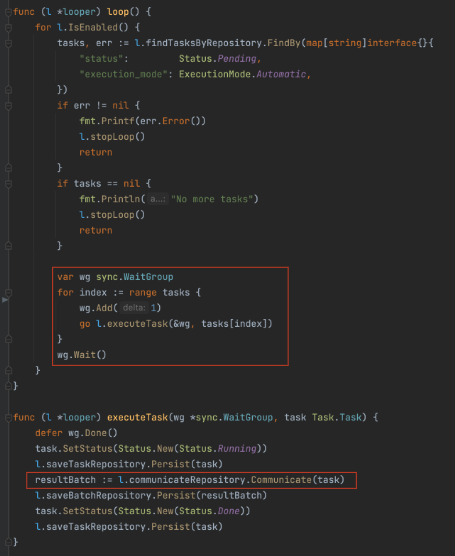
\includegraphics[height=0.3\textheight]{./part/Ejecucion/Seguimiento/Testing/img/Looper}
    \caption{testing looper.go detail}\label{fig:testingLooper}
\end{figure}

el punto clave de la figura \ref{fig:testingLooper} señalado en el recuadro rojo es el adaptador de comunicación GRPC es un adaptador experimental que debido a la inexperiencia en su uso está desarrollado de forma ineficiente. Hemos extraido toda la lógica posible a este servicio que es la parte core:

El adaptador puede tener múltiples errores inesperados, no conseguir comunicar con el servicio cliente, timeouts, malas implementaciones de la librería, pero se ha protegido al dominio de todo esto mediante una interfaz que garantiza que ante cualquier error se devuelve siempre un resultado. Lo único que quedaría por implementar y testear sería que el proceso no consiguiera terminar y se quedara la gorutine en un proceso infinito. para ello en el proceso de descubrimiento del lenguaje sabemos que hay un punto débil en el dominio. No hemos hehco uso de una herramienta de Golang que se conoce como context. que permite gestionar los timeouts de las gorutines evitando que que queden procesos hijos sin control.

Tengamos en cuenta que hemos extraido de toda la comunicación con el cliente una interfaz útil y única para comunicarnos, una lógica de negocio que entender en pocas lineas de código y explicar su funcionamiento, controlarlo y testearlo y aún así encontramos puntos débiles que mejorar en ese diseño. Si a esto le hubieramos sumado las lineas de codigo que hay detrás de la interfaz de comunicacion sería ingestionable. para cuantificar esto vamos a hacer una aproximación al diseño del test necesario para cubrir el adaptador de comunicacion

El código completo se encuentra en el repositorio github. Simplificando para esta explicación el pseudocódigo sería el siguiente

\begin{verbatim}
connection, err := grpc.Dial()
    serverStream:
        client.CallServerStream(request)
        responseStream.Recv()
    Bidirectional:
        client.CallBidirectional()
        async stream.Recv()
        async stream.Send()
        stream.CloseSend()
    ClientStream:
        client.CallClientStream()
        stream.Send
        stream.CloseAndRecv()
    Unary
        client.CallUnary()
connection.Close()
\end{verbatim}

vemos que hay mucha lógica junta, múltiples responsabilidades y por lo tanto no es un buen diseño. Como se demuestra mejor es intentando diseñar los tests. Para empezar extraer del código estas clases de equivalencia y factores no ha sido sencillo ya que hay multiples gestiones de errores dispersos por el código y es un código extenso 178 lineas. Esto ocurre en multitud de ocasiones, ya sea debido al tiempo, desconocimiento o mala praxis nos encontramos con códigos de esta magnitud. La arquitectura y todo este proceso lo que hace es protegernos de estas secciones sucias.

factores y posibles respuestas:

\begin{itemize}
    \item grpc.Dial(): err, connection
    \item client.CallServerStream(request): err,stream
    \item responseStream.Recv(): EOF,err,nil
    \item client.CallBidirectional(): error,stream
    \item stream.Recv(): EOF,err, result
    \item stream.Send(): EOF, nil,err
    \item stream.CloseSend() err,nil
    \item client.CallClientStream(): err, stream
    \item stream.Send: err, nil
    \item stream.CloseAndRecv(): err, nil
    \item client.CallUnary(): err,nil
    \item connection.Close(): err, nil
\end{itemize}

Si no entendieramos bien el concepto de clase de equivalencia podría llevarnos a un mal diseño de los tests o a hacerlo más complejo. Aunque hay factores que tiene tres respuestas posibles EOF y nil tienen que ir de la mano, significa que no ha habido error, primero obtienes un nil en el error y luego obtienes un error tipo EOF que significa que todo ha terminado correctamente. y luego tenemos cuando obtenmos un error distinto de EOF, si esto ocurre nos importa cuaántas veces haya ocurrido el caso sin error, será error igualmente. Con lo cual las clases de equivalencia serían

\begin{itemize}
    \item grpc.Dial(): err, connection
    \item client.CallServerStream(): err,stream
    \item responseStream.Recv(): nil\&EOF,err
    \item client.CallBidirectional(): error,stream
    \item stream.Recv(): nil\&EOF,err
    \item stream.Send(): nil\&EOF,err
    \item stream.CloseSend() err,nil
    \item client.CallClientStream(): err, stream
    \item stream.Send: err, nil
    \item stream.CloseAndRecv(): err, nil
    \item client.CallUnary(): err,nil
    \item connection.Close(): err, nil
\end{itemize}

para este caso tendríamos \[ 2^{12} = 4096 \] combinaciones posibles que pairwise reduce a 59 tests. aquí se ve la potencia del método. Volviendo posible un testing con ciertas garantías incluso en un código como el que nos ocupa.

\subsubsection{Puesta a punto y resultados}
    
\subsubsection{Pipeline}

En el proceso de Pull Request, tal y como se diseño~\nameref{par:testing}, se ejecuta el pipeline diseñado para garantizar la entrega de software testeado y con el estandar de calidad requerido.
Podemos ver en la figura~\cref{fig:githubActions} que los pasos son:

\begin{itemize}
    \item ejecutar los tests
    \item pasar el chequeo de estandar del código
    \item compilar en modo producción
\end{itemize}

faltarían el CD o continous delivery que ejecutaría los pasos de subir dicho ejecutable a un servidor, al menos para el programa manager.

\begin{figure}[H]
    \centering
    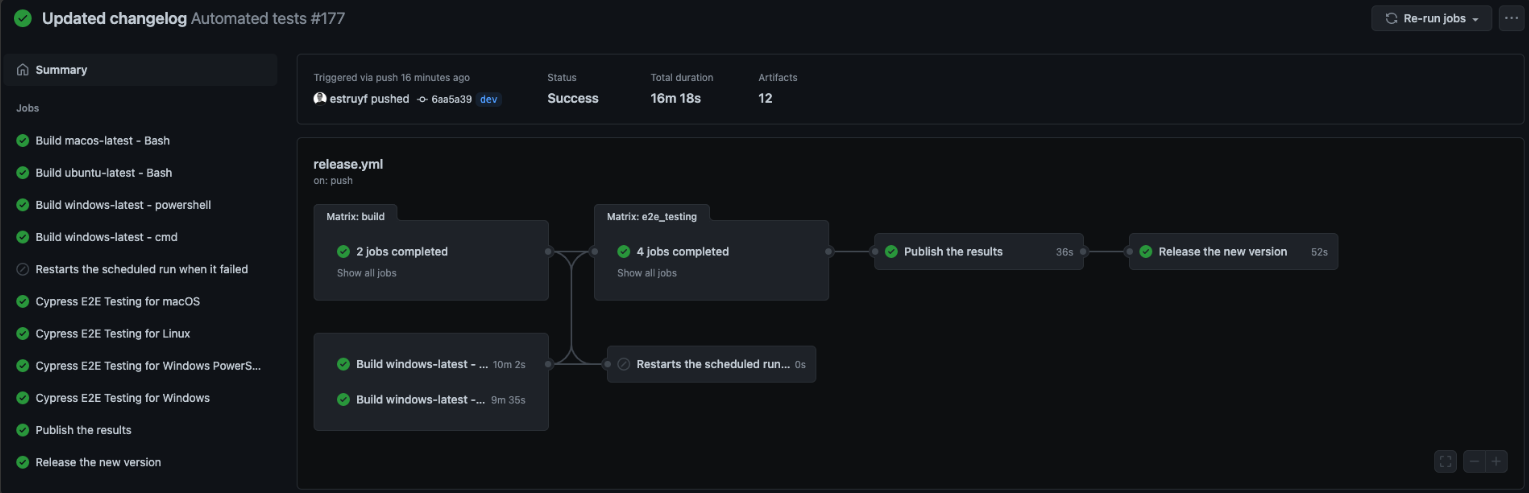
\includegraphics[height=0.2\textheight]{./part/Ejecucion/Seguimiento/PuestaAPunto/img/githubPipelines}
    \caption{Pipeline en Github}\label{fig:githubActions}
\end{figure}

\subsubsection{Montaje de prueba}

Para la prueba conjunta del sistema se ha desplegado un montaje como se ve en la figura~\cref{fig:Control-Diagrama UML de despliegue}

\begin{figure}[H]
    \centering
    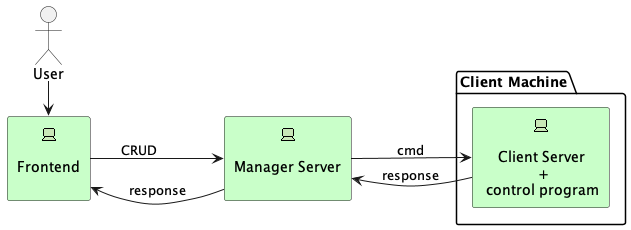
\includegraphics[height=0.2\textheight]{./part/Ejecucion/Seguimiento/PuestaAPunto/img/deploy}
    \caption{Diagrama de despliegue de prueba}\label{fig:despliegue de prueba}
\end{figure}

La imagen~\cref{fig:montaje en protoboard} muestra el montaje físico de conexión entre el el servidor cliente.
La Raspberry se conecta en una protoboard donde se realiza la conexión con el puente H y el motor de corriente continua.

\begin{figure}[H]
    \centering
    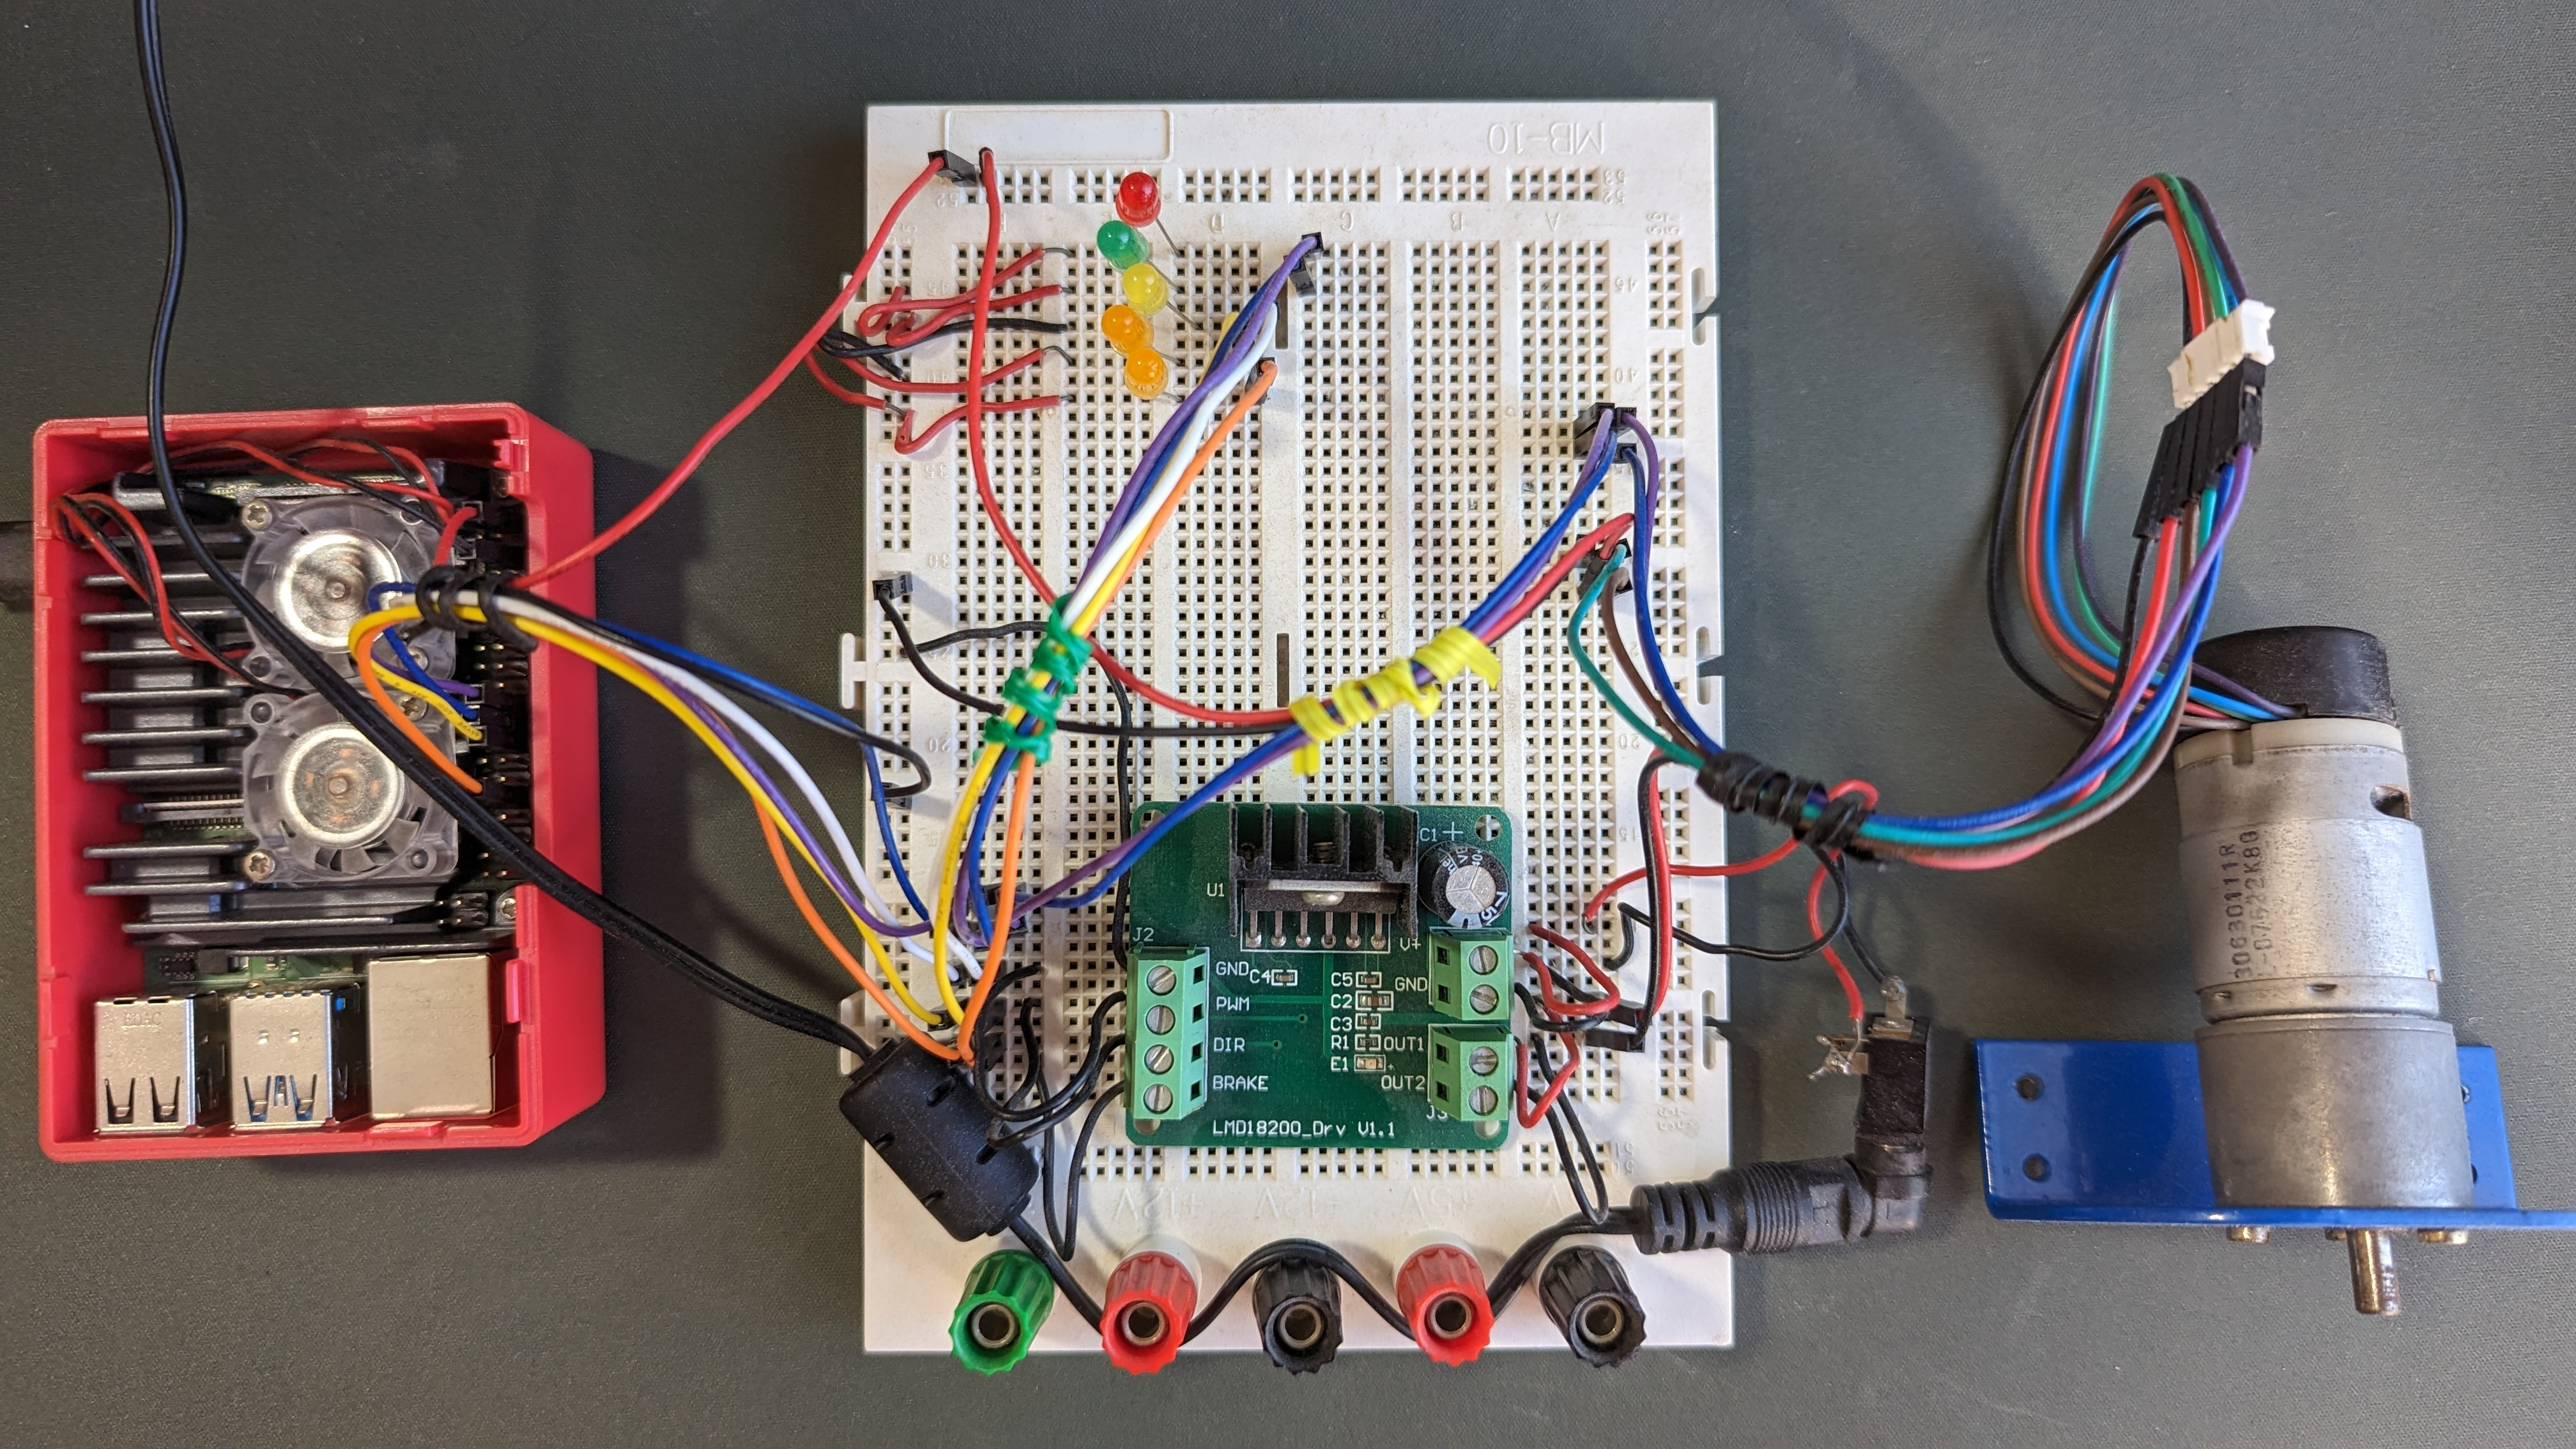
\includegraphics[height=0.2\textheight]{./part/Ejecucion/Seguimiento/PuestaAPunto/img/montajeProtoboard}
    \caption{Montaje en protoboard}\label{fig:montaje en protoboard}
\end{figure}

\subsubsection{Interfaz gráfica}

Para controlar el programa manager se ha desarrollado como añadido una interfaz gráfica.
En la figura~\cref{fig:frontend} podemos ver el listado de las tareas creadas, el estado en el que se encuentran y un boton para ejecutar manualmente las que son manuales.
Para ejecutar manualmente una tarea disponimos de una gráfica para ver en tiempo real la evolución de la variable controlada tal y como podemos ver en el~\cref{fig:runner}

\begin{figure}[H]
    \centering
    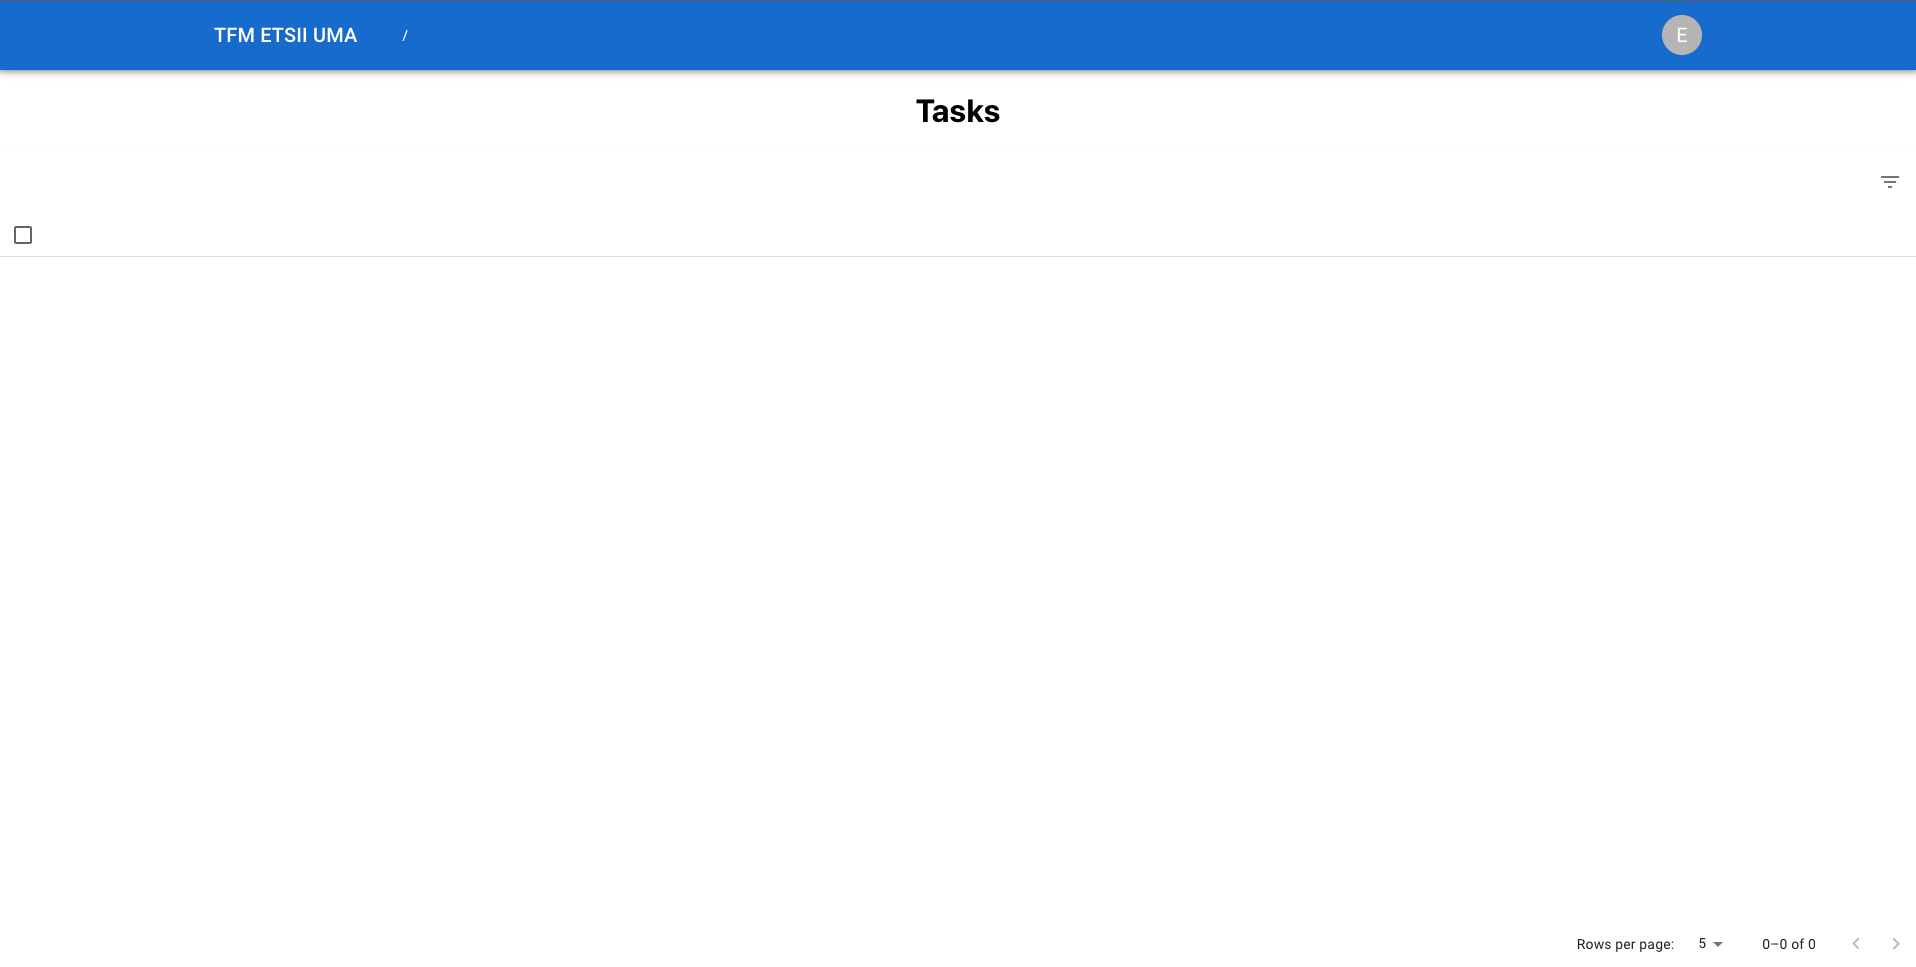
\includegraphics[height=0.2\textheight]{./part/Ejecucion/Seguimiento/PuestaAPunto/img/frontend}
    \caption{Frontend: task list}\label{fig:frontend}
\end{figure}

\begin{figure}[H]
    \centering
    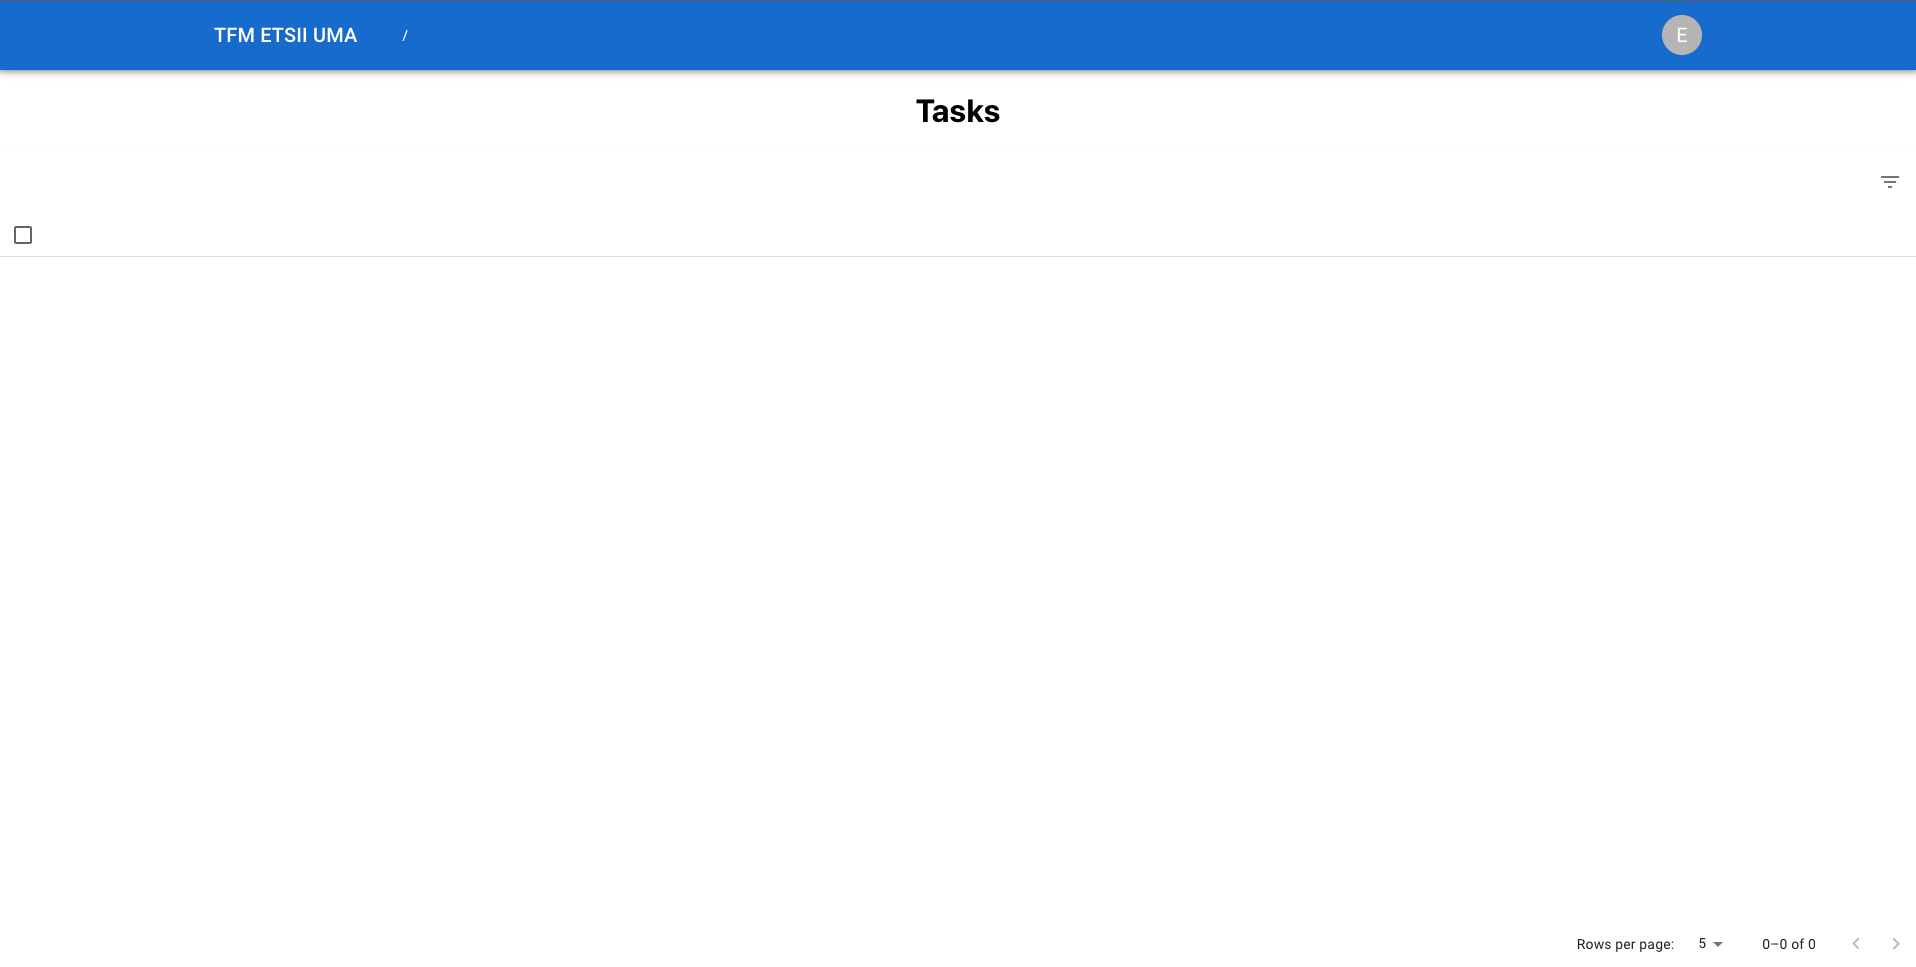
\includegraphics[height=0.2\textheight]{./part/Ejecucion/Seguimiento/PuestaAPunto/img/runner}
    \caption{Frontend: runner}\label{fig:runner}
\end{figure}


